\documentclass[12pt]{beamer}
\usepackage{amsmath}
\usepackage{mathtools}
\usepackage{multimedia}
\usepackage{hyperref}
\usepackage{booktabs}
\usepackage[T1]{fontenc}
\usepackage{tikz}

\usefonttheme{professionalfonts} % using non standard fonts for beamer
\usefonttheme{serif} % default family is serif
%\documentclass[12pt]{beamerthemeSam.sty}
\usepackage{epsf}
%\usepackage{pstricks}
%\usepackage[orientation=portrait,size=A4]{beamerposter}
\geometry{paperwidth=160mm,paperheight=120mm}
%DT favorite definitions
\def\LL{\left\langle}	% left angle bracket
\def\RR{\right\rangle}	% right angle bracket
\def\LP{\left(}		% left parenthesis
\def\RP{\right)}	% right parenthesis
\def\LB{\left\{}	% left curly bracket
\def\RB{\right\}}	% right curly bracket
\def\PAR#1#2{ {{\partial #1}\over{\partial #2}} }
\def\PARTWO#1#2{ {{\partial^2 #1}\over{\partial #2}^2} }
\def\PARTWOMIX#1#2#3{ {{\partial^2 #1}\over{\partial #2 \partial #3}} }

\def\rightpartial{{\overrightarrow\partial}}
\def\leftpartial{{\overleftarrow\partial}}
\def\diffpartial{\buildrel\leftrightarrow\over\partial}

\def\HC{\column{0.5\textwidth}}
\def\BBC{\begin{columns}}
\def\EEC{\end{columns}}
\def\BCC{\begin{columns}}
\def\ECC{\end{columns}}
\def\BC{\begin{center}}
\def\EC{\end{center}}
\def\BN{\begin{enumerate}}
\def\EN{\end{enumerate}}
\def\BI{\begin{itemize}}
\def\EI{\end{itemize}}
\def\BE{\begin{displaymath}}
\def\EE{\end{displaymath}}
\def\BEA{\begin{eqnarray*}}
\def\EEA{\end{eqnarray*}}
\def\BNEA{\begin{eqnarray}}
\def\ENEA{\end{eqnarray}}
\def\EL{\nonumber\\}

\newcommand{\etal}{{\it et al.}}
\newcommand{\gbeta}{6/g^2}
\newcommand{\la}[1]{\label{#1}}
\newcommand{\ie}{{\em i.e.\ }}
\newcommand{\eg}{{\em e.\,g.\ }}
\newcommand{\cf}{cf.\ }
\newcommand{\BS}{\bigskip}
\newcommand{\etc}{etc.\ }
\newcommand{\atantwo}{{\rm atan2}}
\newcommand{\Tr}{{\rm Tr}}
\newcommand{\dt}{\Delta t}
\newcommand{\op}{{\cal O}}
\newcommand{\msbar}{{\overline{\rm MS}}}
\def\chpt{\raise0.4ex\hbox{$\chi$}PT}
\def\schpt{S\raise0.4ex\hbox{$\chi$}PT}
\def\MeV{{\rm Me\!V}}
\def\GeV{{\rm Ge\!V}}

%AB: my color definitions
%\definecolor{mygarnet}{rgb}{0.445,0.184,0.215}
%\definecolor{mygold}{rgb}{0.848,0.848,0.098}
%\definecolor{myg2g}{rgb}{0.647,0.316,0.157}
\definecolor{A}{rgb}{1.0,0.3,0.3}
\definecolor{B}{rgb}{0.0,1.0,0.0}
\definecolor{C}{rgb}{1.0,1.0,0.0}
\definecolor{D}{rgb}{0.5,0.5,1.0}
\definecolor{E}{rgb}{0.7,0.7,0.7}
\definecolor{abtitlecolor}{rgb}{1.0,1.0,1.0}
\definecolor{absecondarycolor}{rgb}{0.0,0.416,0.804}
\definecolor{abprimarycolor}{rgb}{1.0,0.686,0.0}
\definecolor{Red}           {rgb}{1,0.4,0.4}
\definecolor{Yellow}           {rgb}{1,1,0.0}
\definecolor{Grey}          {cmyk}{.7,.7,.7,0}
\definecolor{Blue}          {cmyk}{1,1,0,0}
\definecolor{Green}         {cmyk}{1,0,1,0}
\definecolor{Brown}         {cmyk}{0,0.81,1,0.60}
\definecolor{Silver}        {rgb}{0.95,0.9,1.0}
\definecolor{Sky}           {rgb}{0.07,0.0,0.2}
\definecolor{Darkbrown}     {rgb}{0.4,0.3,0.2}
\definecolor{Black}         {rgb}{0.0,0.0,0.0}
\definecolor{Orange}         {rgb}{1.0,0.5,0.0}
\definecolor{40Gray}        {rgb}{0.4,0.4,0.5}
\usetheme{Madrid}


\setbeamercolor{normal text}{fg=Silver,bg=Sky}

%AB: redefinition of beamer colors
%\setbeamercolor{palette tertiary}{fg=white,bg=mygarnet}
%\setbeamercolor{palette secondary}{fg=white,bg=myg2g}
%\setbeamercolor{palette primary}{fg=black,bg=mygold}
\setbeamercolor{title}{fg=abtitlecolor}
\setbeamercolor{frametitle}{fg=abtitlecolor}
\setbeamercolor{palette tertiary}{fg=white,bg=Darkbrown}
\setbeamercolor{palette secondary}{fg=white,bg=absecondarycolor}
\setbeamercolor{palette primary}{fg=white,bg=40Gray}
\setbeamercolor{structure}{fg=abtitlecolor}

\setbeamerfont{section in toc}{series=\bfseries}

%AB: remove navigation icons
\beamertemplatenavigationsymbolsempty
\title[Ad astra per aspera, II]{
  \textbf {Ad astra per aspera, II}}

\author [Astronomy 101]{Astronomy 101\\Syracuse University, Fall 2019\\Walter Freeman}

\date{\today}

\begin{document}



\frame{\titlepage}

\frame{
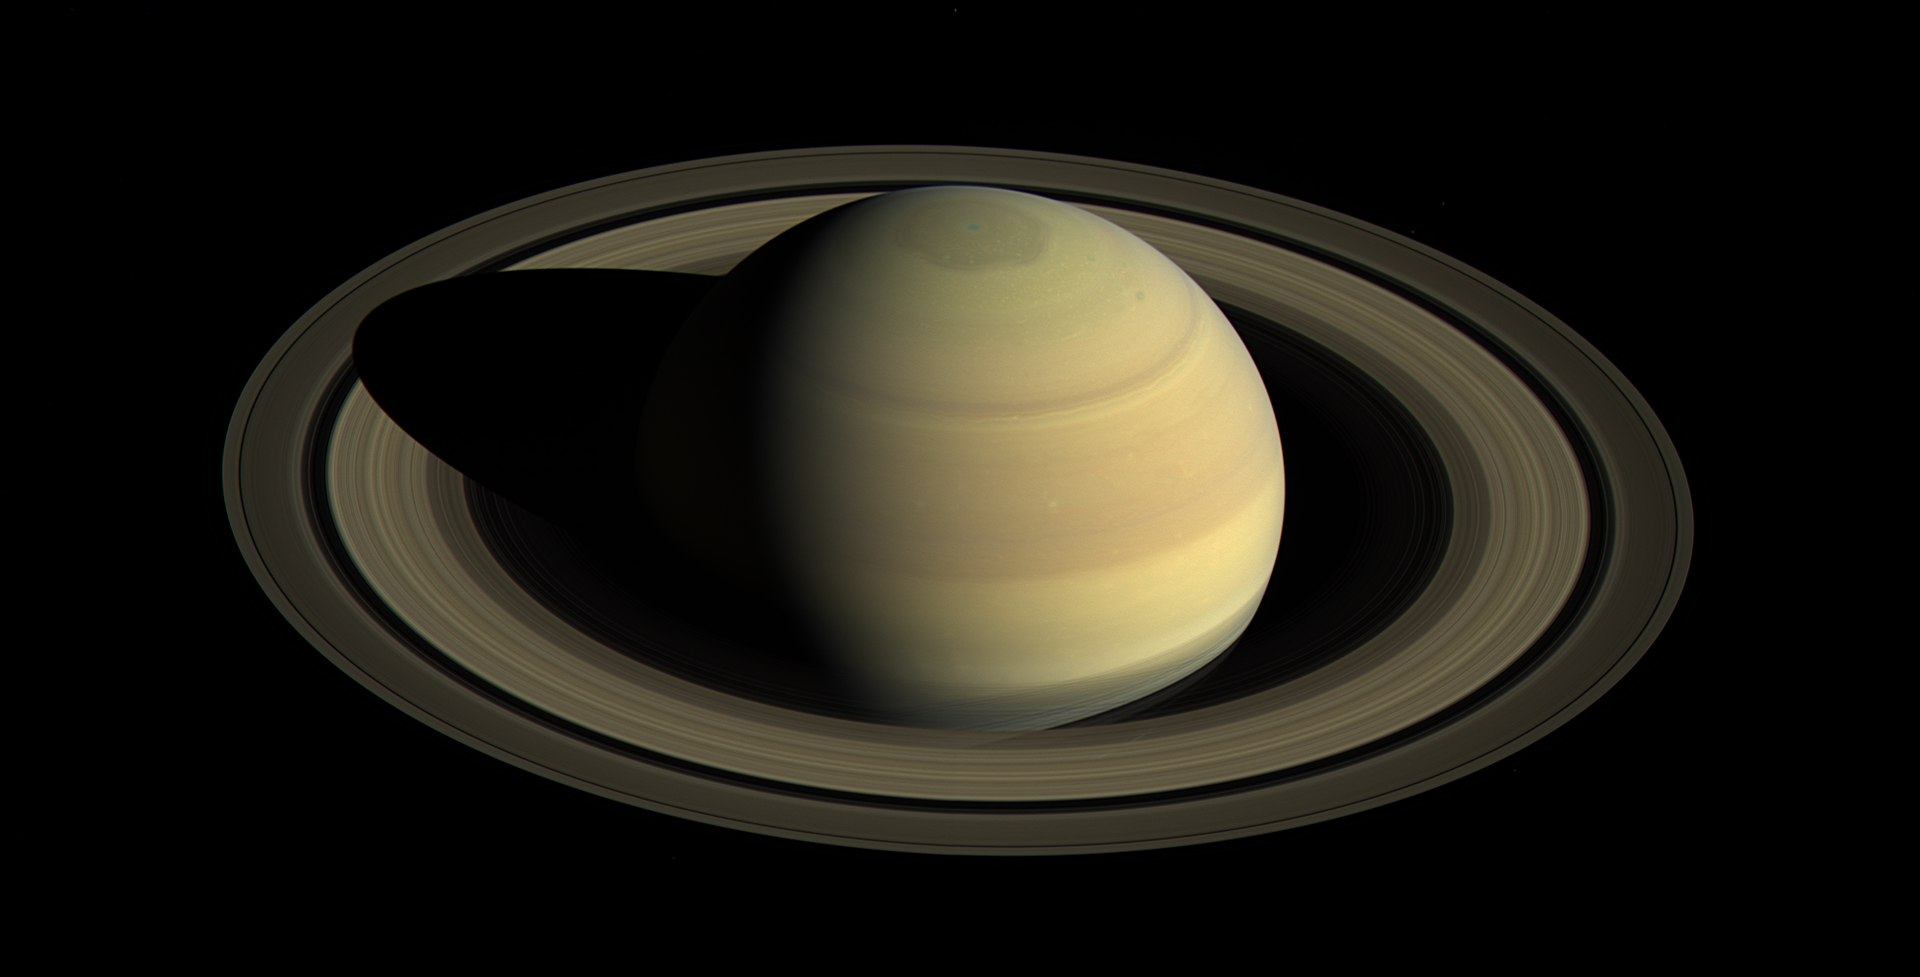
\includegraphics[width=\textwidth]{saturn.jpg}
\BS

\it \small
I still remember when the first time I pointed the telescope at the sky and I saw Saturn with the rings. It was a beautiful image. And that really made my mind to become a scientist. And that was the first step in order to become an astronaut, of course.
\rm
\begin{flushright}--Umberto Guidoni, Italian astronaut, to NASA (2001)\end{flushright}
}

\frame{
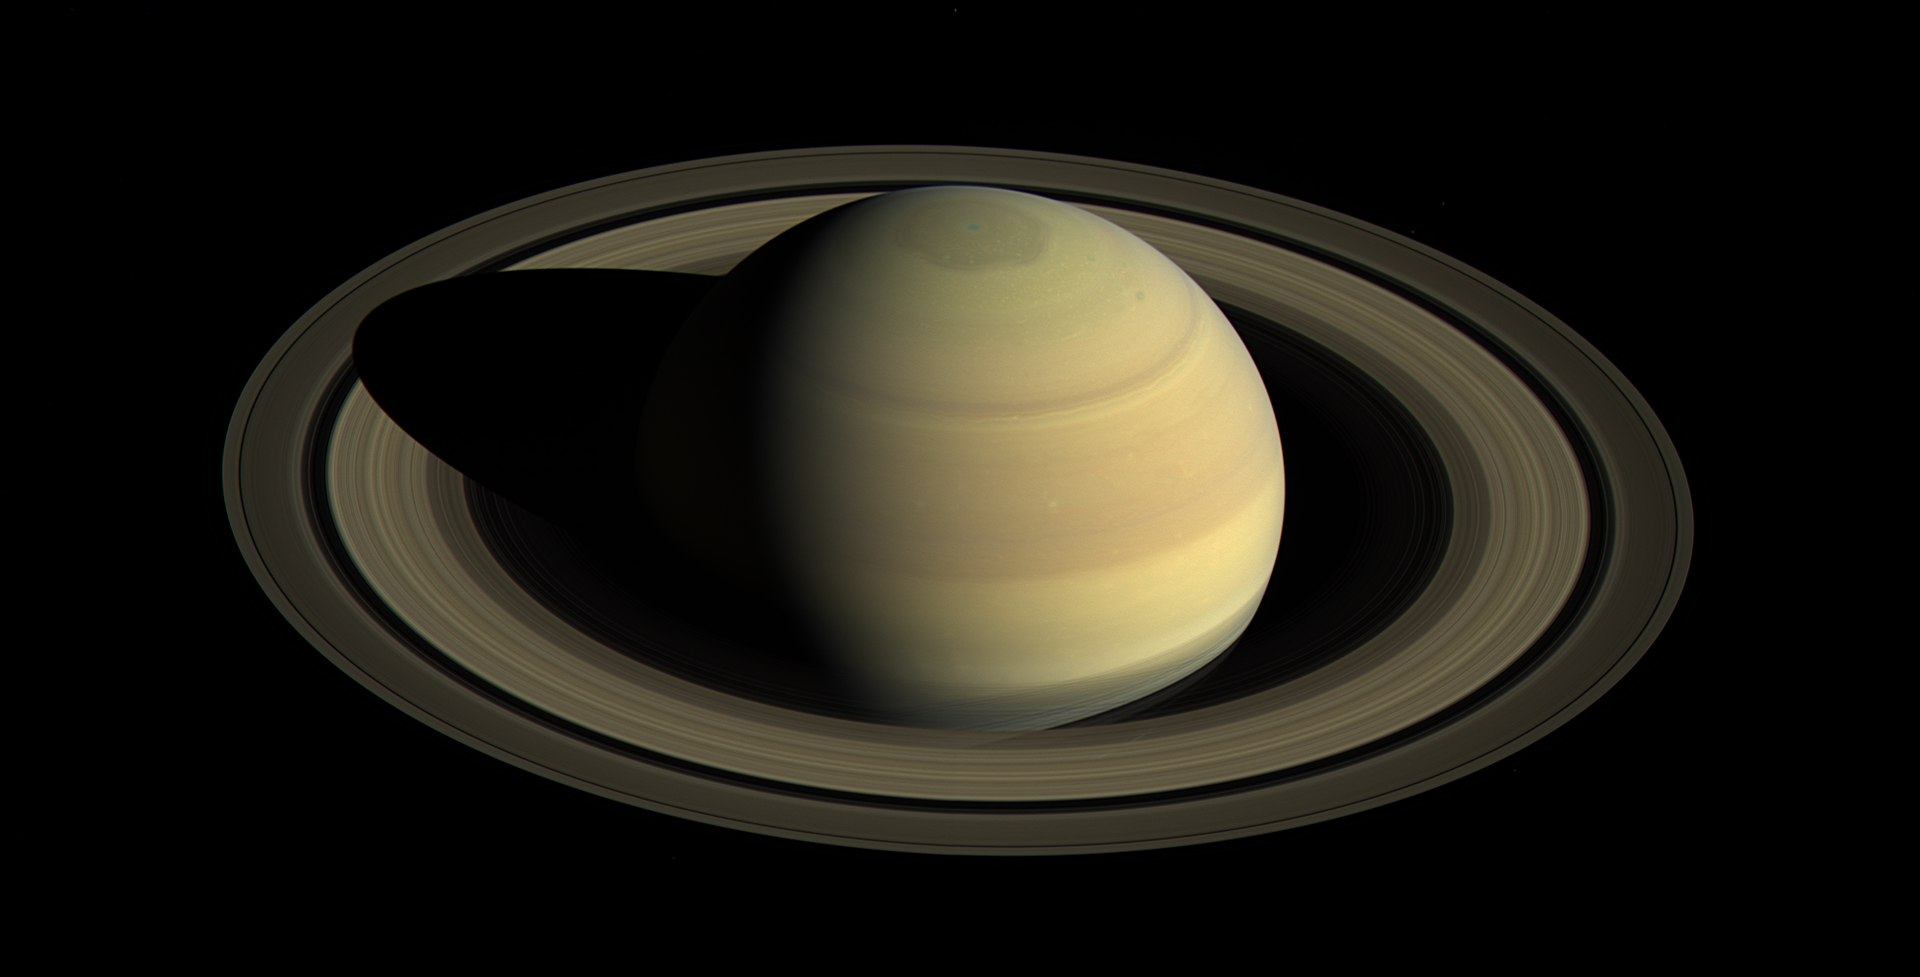
\includegraphics[width=\textwidth]{saturn.jpg}
\BS

\it \small
It's amazing to me that not only can we put a probe around Saturn and get images of its moons, but our math and physics are so freaking accurate we can say, ``Hey, you know what? On this date at this time if we turn Cassini 
that way we’ll see a moon over 2 million kilometers away pass in front of another one nearly 3 million kilometers away.''
Every morning, I have a 50/50 chance of finding my keys. That kinda puts things in perspective.
\rm
\begin{flushright}--Phil Plait, American astronomer (2010)\end{flushright}
}


\frame{\frametitle{\textbf{Announcements}}
\large
Final projects should be turned in:
\BI
\item In office hours tomorrow in my office (9:30-12)
\item In office hours Monday in the Clinic (time TBD)
\item At the makeup lab (but be aware I'll be running around)
\item When you come for the final (preferred)
\item By making special arrangements with me (difficult fine-art type projects)
\item Email for submissions of digital projects: {\tt suast101projects@gmail.com}
\item {\bf If you also turn in a physical copy, add ``backup submission'' to the title of your email.}
\item We would appreciate an email copy of anything that can be 
emailed, in addition to the paper copy.
\EI

}


%
%\frame{\frametitle{\textbf{Announcements}}
%\large
%
%Almost all of your grades are online. I haven't yet gotten to exams that people took as makeups, or papers that I personally will be grading.
%
%\BS
%
%Labs 10 and 11, and Paper 2, may not have been graded yet by TA's. If you have a missing grade, email me and your TA, and:
%
%\normalsize
%
%\BI
%\item {\bf Put ``missing grade'' in the title, along with what is missing}
%\item Tell me what is missing and any unusual circumstances surrounding it
%\item If it's something you got back from your TA, please include a photograph of the paper with your grade
%\item We'll fix it as soon as we can
%\EI
%}


\frame{\frametitle {\bf Preparing for the final exam}
\large
\BI
\item The final exam is {\bf next Tuesday, 3PM - 5PM, 10 December}
\item {\bf Section 1: Stolkin Auditorium (here)} 
\item {\bf Section 2: Grant Auditorium (Falk)} 

\item You may bring handwritten notes of any length, along with your books and 
anything you have written in them. 
\BS\BS
\pause
\item It is likely I will be very very slow answering email Monday and Tuesday, since all of my time will be face-to-face with students.
\pause
\item I'm sorry about this, but I am helping folks as fast as I can.
\item If there is an issue, don't worry -- I will make sure it's resolved fairly.
\EI
}

\frame{\frametitle {\bf Preparing for the final exam: review sessions}
\large
\BI
\item Friday: in my office from 9:30-12
\item Friday: I'll be in Holden from 2pm-11pm doing makeup labs (you can come for other things too)
\item Next Monday: in the Physics Clinic from 12-3, and maybe other times as well
\item Next Tuesday: will be in and out of the Physics Clinic from 10AM until your exam starts
\pause
\item I will be giving priority to people with {\it science questions} (exams, projects) at my office hours
\EI
}


\frame{\frametitle{\bf Summary}
\large
Last time:

\BI
\item {\bf Since the end of human flight to the Moon in 1972, we've not been there or anywhere else interesting}
\pause
\item We've gotten very good at robots: to orbit, to the planets (especially Mars), and out of the Solar System
\pause
\item {\bf \color{Red}... what now?}
\EI
\BS\BS

\BBC
\HC

The possibility of {\color{Red} life on other worlds...}

\normalsize

\BI
\item What it might look like
\item Where it might be hiding, and how we might find it
\item How likely this is
\EI
\pause
\HC
\large
The possibility of {\color{Red} extraterrestrial civilizations...}
\normalsize
\BI
\item How we might talk to them 
\item What {\it they} might look like
\item How likely {\it they} are: the Drake equation
\EI

\EEC

}


\frame{\frametitle{\bf Summary}
\BBC
\HC
\BC
\large
\vspace{-0.5in}
...How humans might travel throughout the Solar System...
\EC
\normalsize
\BI
\item More time (``work longer'') 
\item More effort (``work harder'')
\item Better rockets (``work smarter'')
\EI
\pause


\HC
\large
\BC
How we might get to the stars 
\EC
\normalsize
\BI
\item The possibility of sending probes to Alpha Centauri 
\item What we might find there
\pause
\item How such a mission might look: patience... 
\EI

\EEC
\BS\BS
\large
\BC
{\color{Red}\it Ad astra per aspera}: how {\it we} might become a spacefaring civilization!

\BI
\normalsize
\item Can we travel to Alpha Centauri? 
\item ... the technical challenges
\item ... the social challenges
\item ... the philosophical challenges
\item ... and how they would change our humanity
\EI
\EC
}

\frame{

\BCC
\HC
\BC
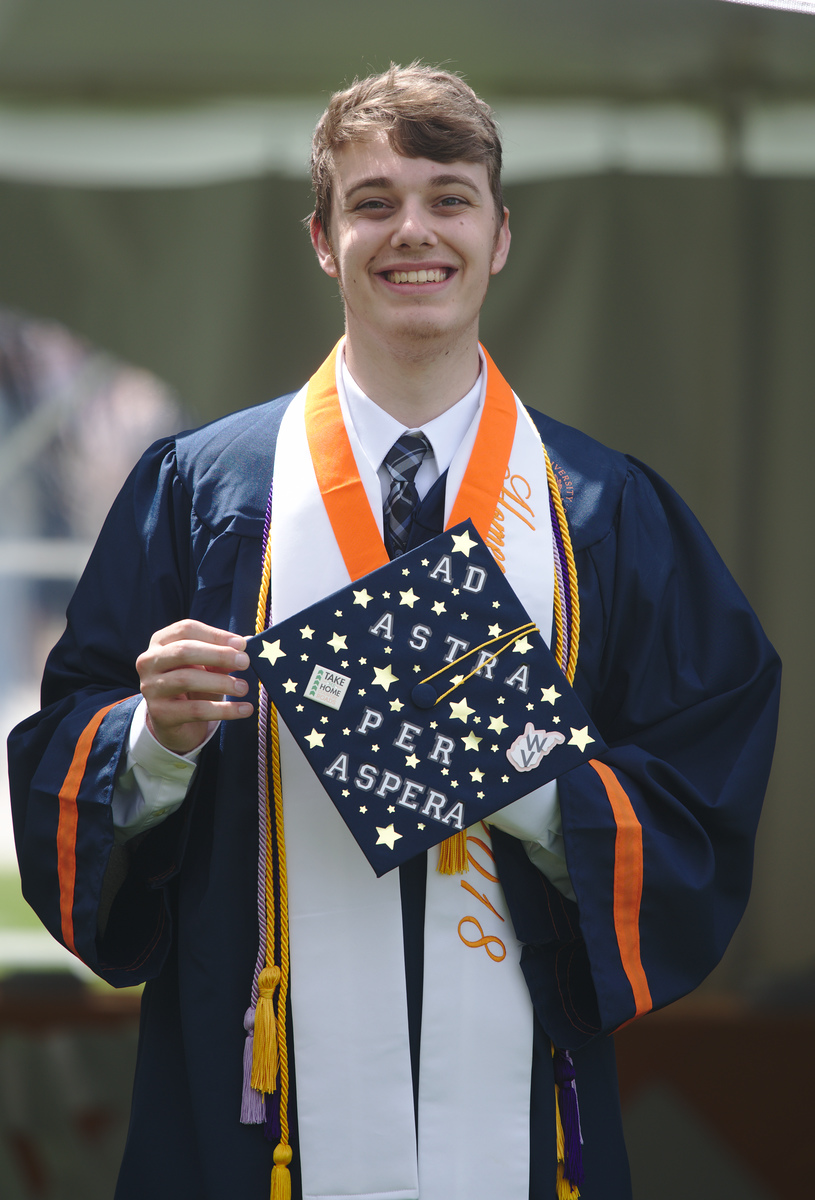
\includegraphics[height=0.95\textheight]{evan.jpg}
\EC
\HC
\large
\begin{center}
	Evan Lewis, BS in Physics, 2019\\
	
	\normalsize
	
	\BS
	College of Arts and Sciences Scholar \\
	
	\BS
	
	Member of the SU Marching Band\\
	
	\BS
	
	Member of the SU Homecoming Court\\
	
	\BS
	
	AST 101 (and PHY 307 and PHY 211) coach\\
	\BS
	Evan is now working toward his PhD in astrophysics (if I recall, in radio astronomy)
\end{center}
\ECC
}

\frame{
	
	\BCC
	\HC
	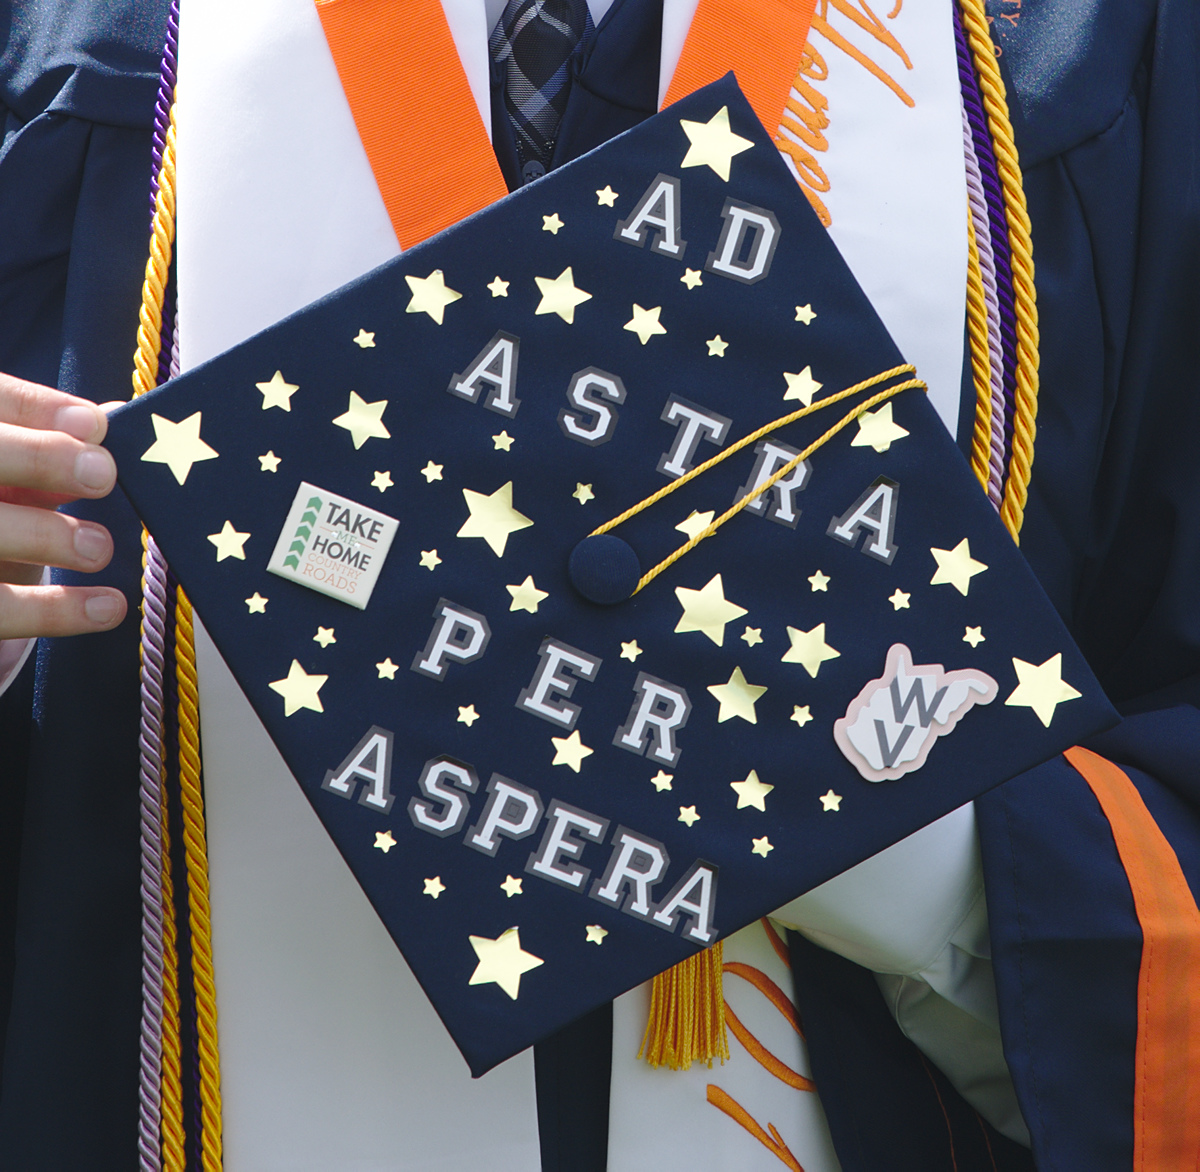
\includegraphics[width=0.95\textwidth]{cap.jpg}
	\HC
	\large
	\begin{center}
		Evan Lewis, BS in Physics, 2019\\
		
		{\color{Red}``Ad astra per aspera''}
		
		\BS\BS\pause
		
		{\color{Green} ``Through hardship, to the stars!''}
		
		\normalsize
		
		\pause\BS\BS
		
		\it(Evan will require less hardship than the rest of us, since he is already so tall.)
		
	\end{center}
	\ECC
}

\frame{\frametitle{\bf Exobiology: life on other worlds}
If we're looking for life elsewhere, we should start by looking for Earth-like life:
\BS
\BI
\normalsize
\item Chains of carbon atoms as structural building blocks: \url{http://bit.ly/2hitrhM}
\item Many different chemical pathways to harnessing energy
\BI
\item Oxygen: very reactive, very handy, not necessary
\item Light: a great primary energy source, but not necessary!
\item Can also metabolize other things: sulfur, iron, manganese...
\EI
\EI
\BC
\BS
\large Life on Earth is much more resilient than we think!
\EC 
\normalsize
\BBC
\HC
\BI
\small
\item Above 200F
\item Below 0F
\item In acid as strong as lemon juice
\item Inside the reactors at Chernobyl (!)
\item Below the deepest oceans
\item On the slopes of Everest
\EI
\HC
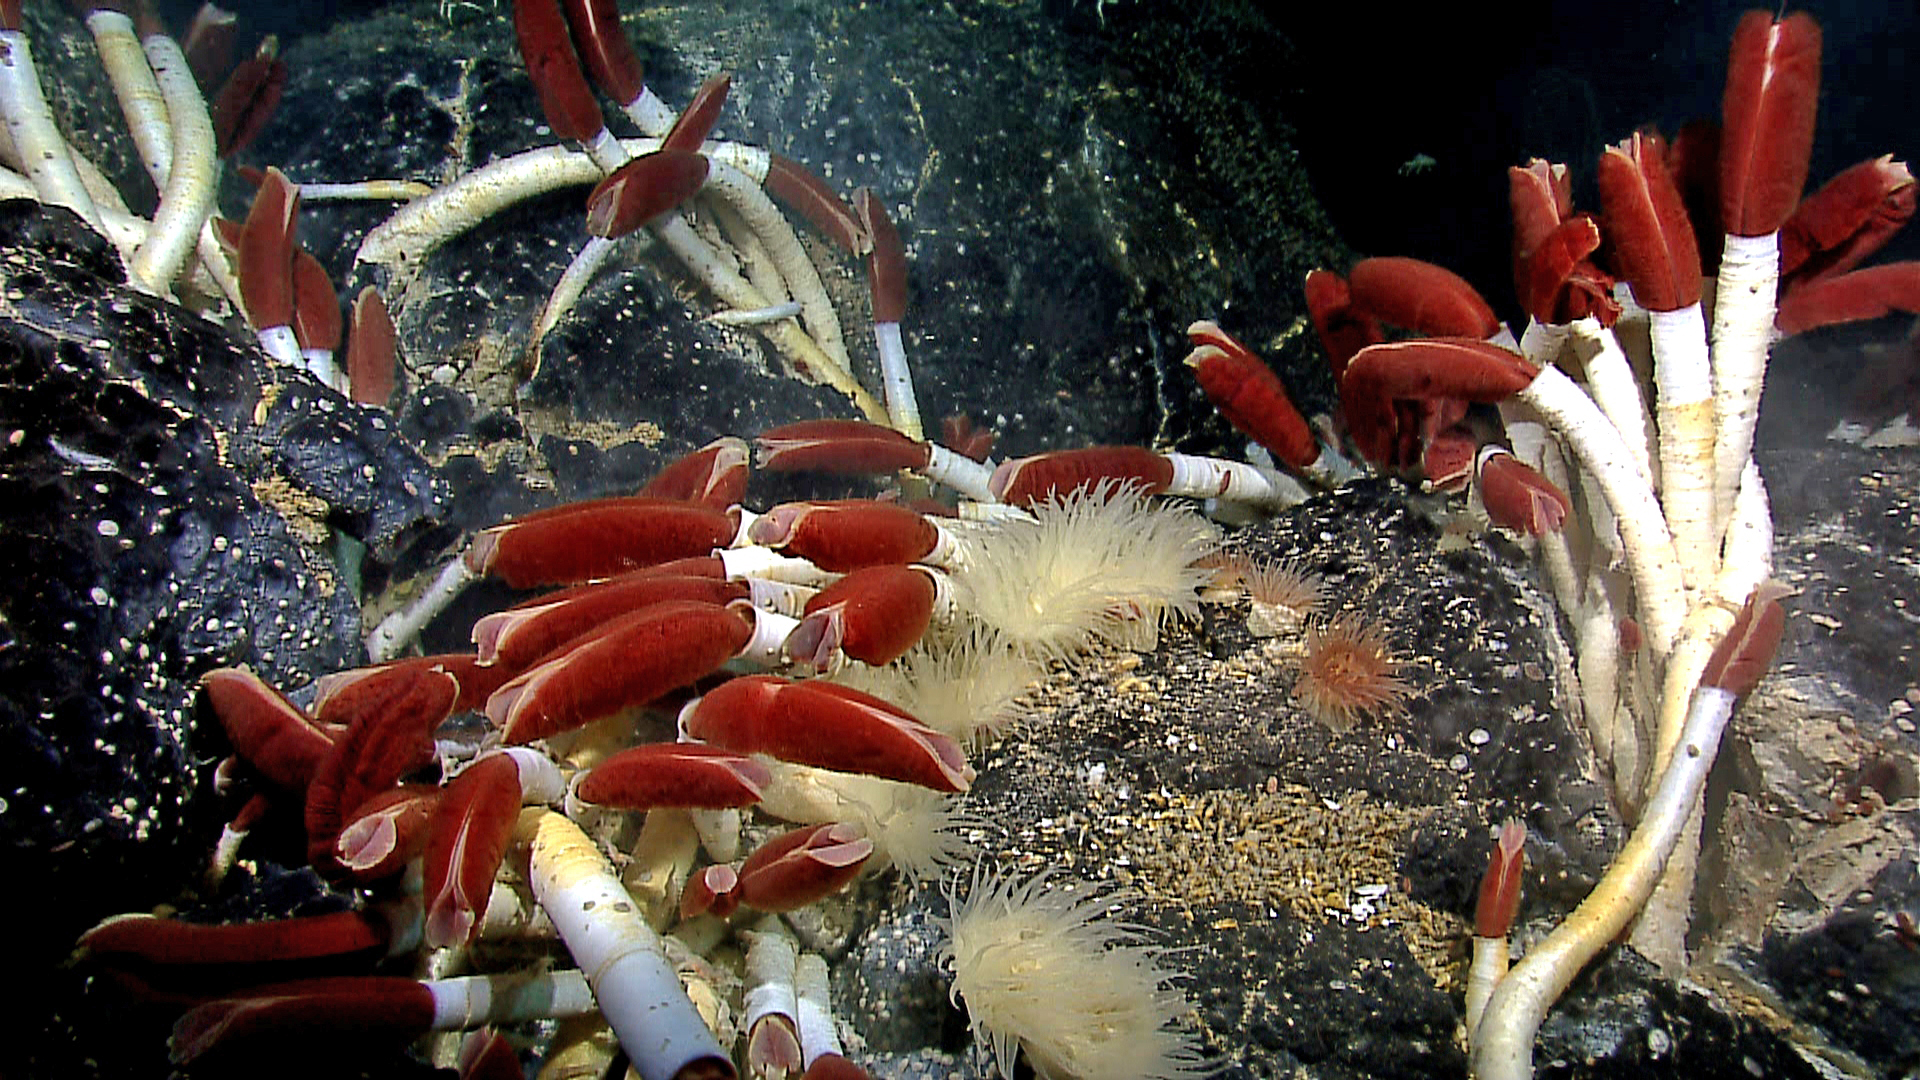
\includegraphics[width=0.9\textwidth]{tube-worms.jpg}
\EEC
}




\frame{\frametitle{\bf Exobiology: the search for water}
\BC
\large
Life on Earth needs liquid water; it allows molecules to float around and find each other
\EC

\BS
\BBC
\HC
Liquid water in the Solar System:

\BI
\item Need temperatures from 0-c. 100 C
\item Earth is perfect (we knew that)
\item Young Mars?
\item The moons of Jupiter and Saturn...
\EI
         
\HC
\BC
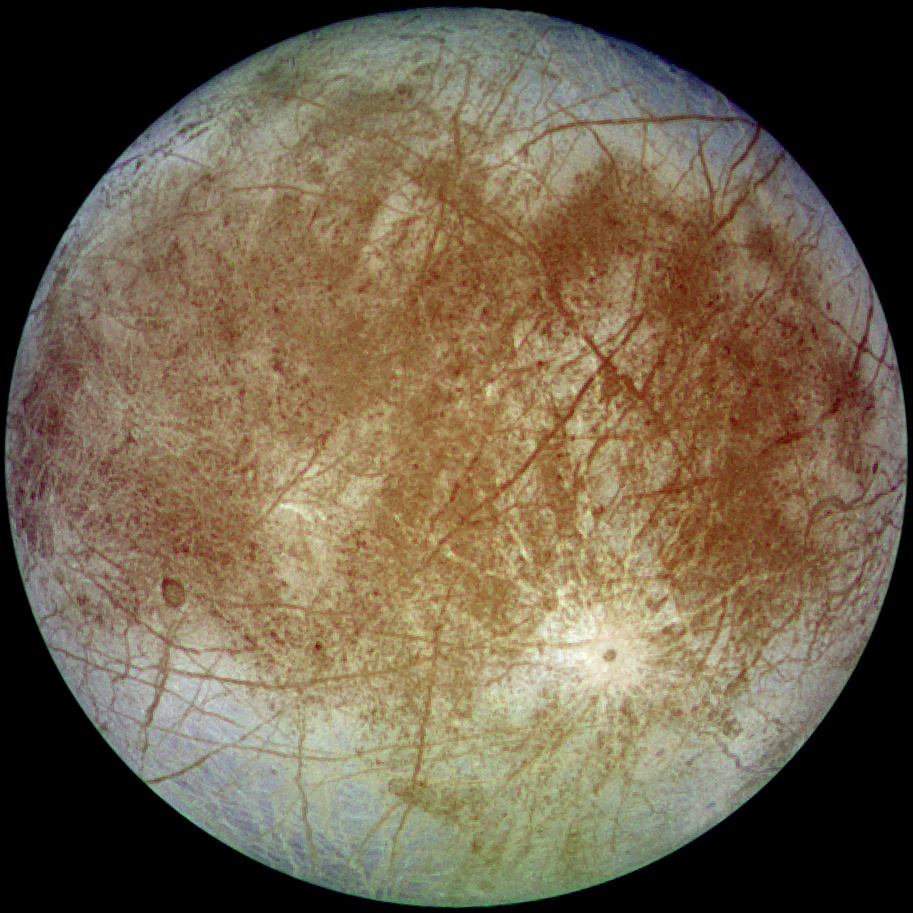
\includegraphics[width=.9\textwidth]{europa.jpg}\\
\it \footnotesize Europa, from the \rm Galileo \it craft (1996)
\EC
\EEC
}



\frame{\frametitle{\bf Enceladus}
\BC
\normalsize There are saltwater oceans under the ice -- and plumes of gas coming out of it!

\BS

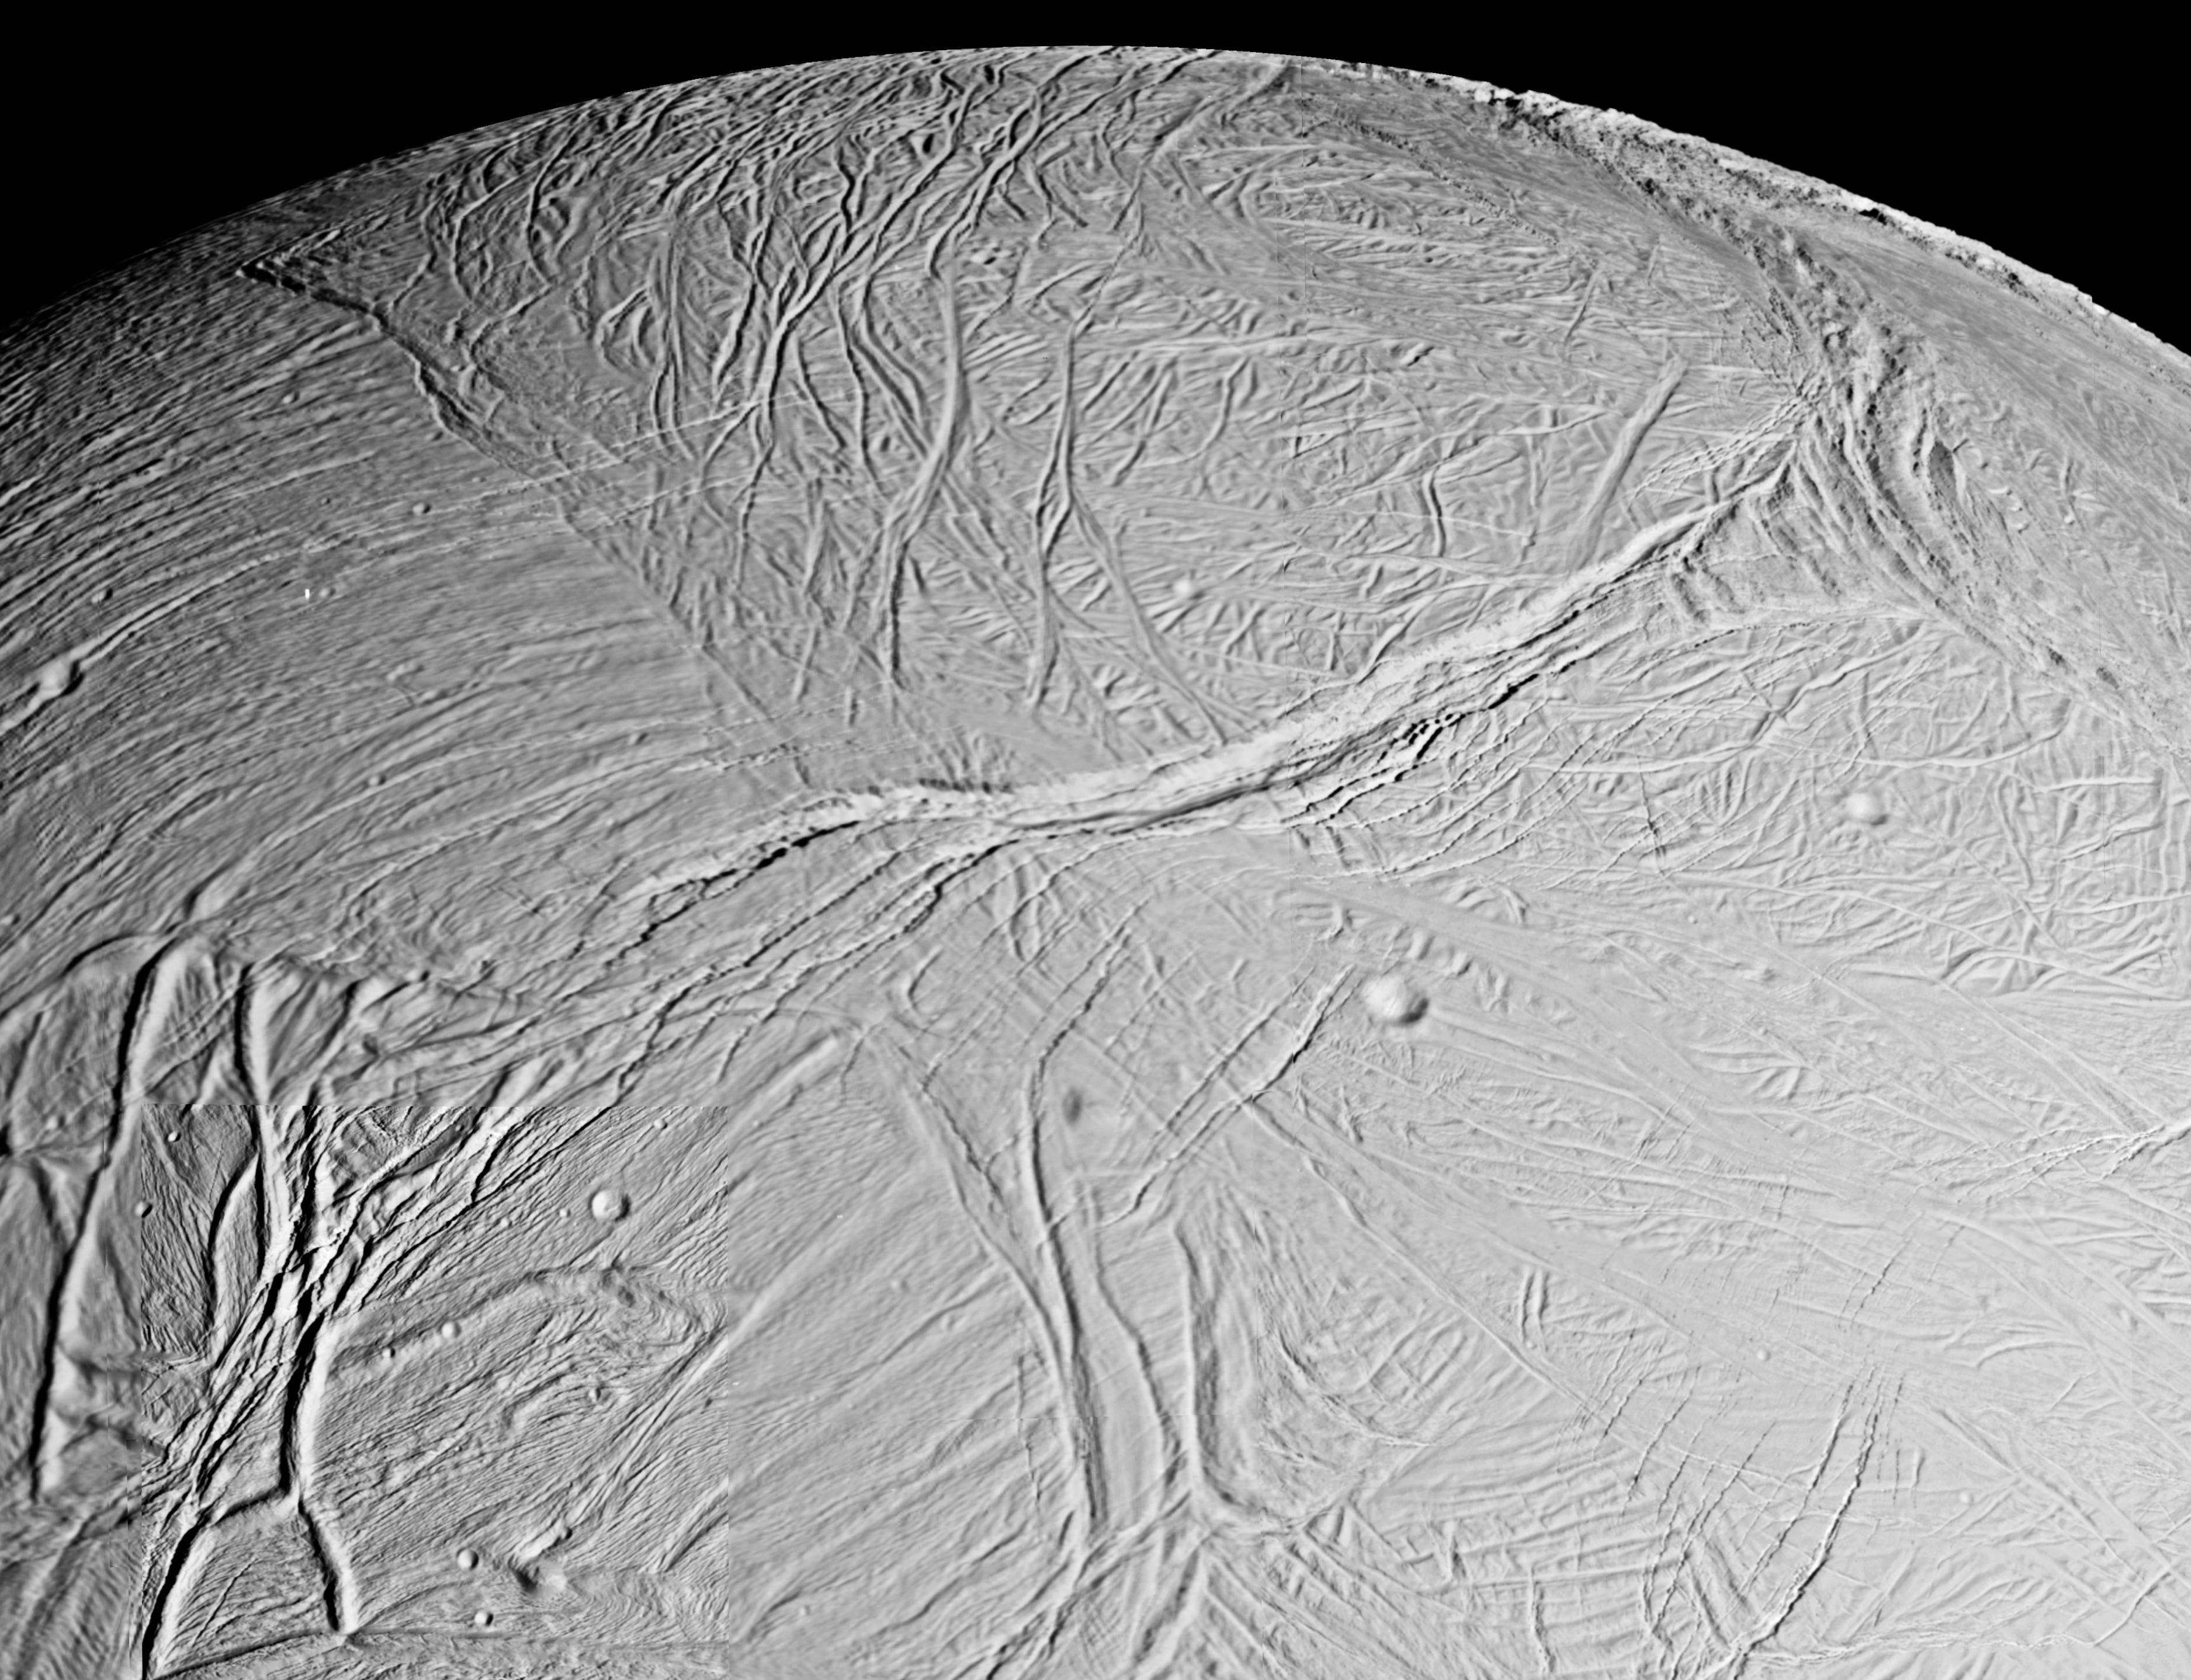
\includegraphics[width=0.7\textwidth]{enceladus.jpg}

\it (From \rm Cassini\it, 2005)

\EC
}


\frame{\frametitle{\bf Enceladus}
\BC
\normalsize What's in them? 

\BS

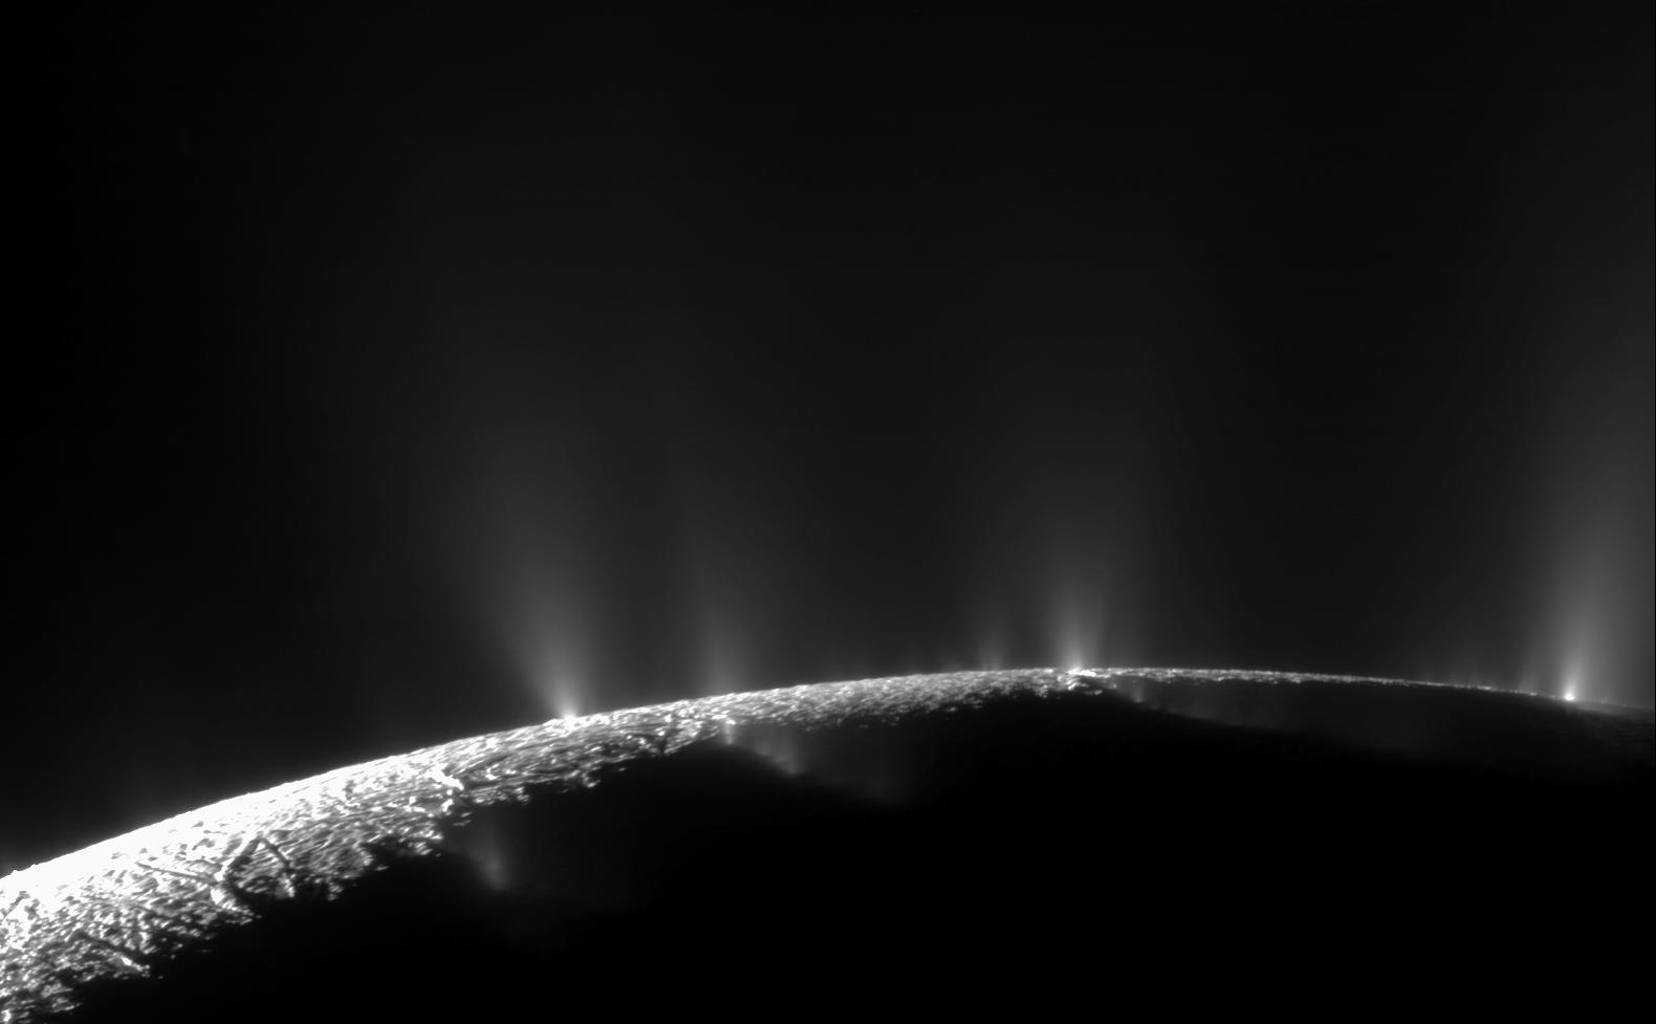
\includegraphics[width=0.9\textwidth]{enceladus-3.jpg}

\it (From \rm Cassini\it, 2009)

\EC
}

\frame{\frametitle{\bf Enceladus}
\BC
\normalsize June, 2018: large organic molecules in these plumes!

\BS

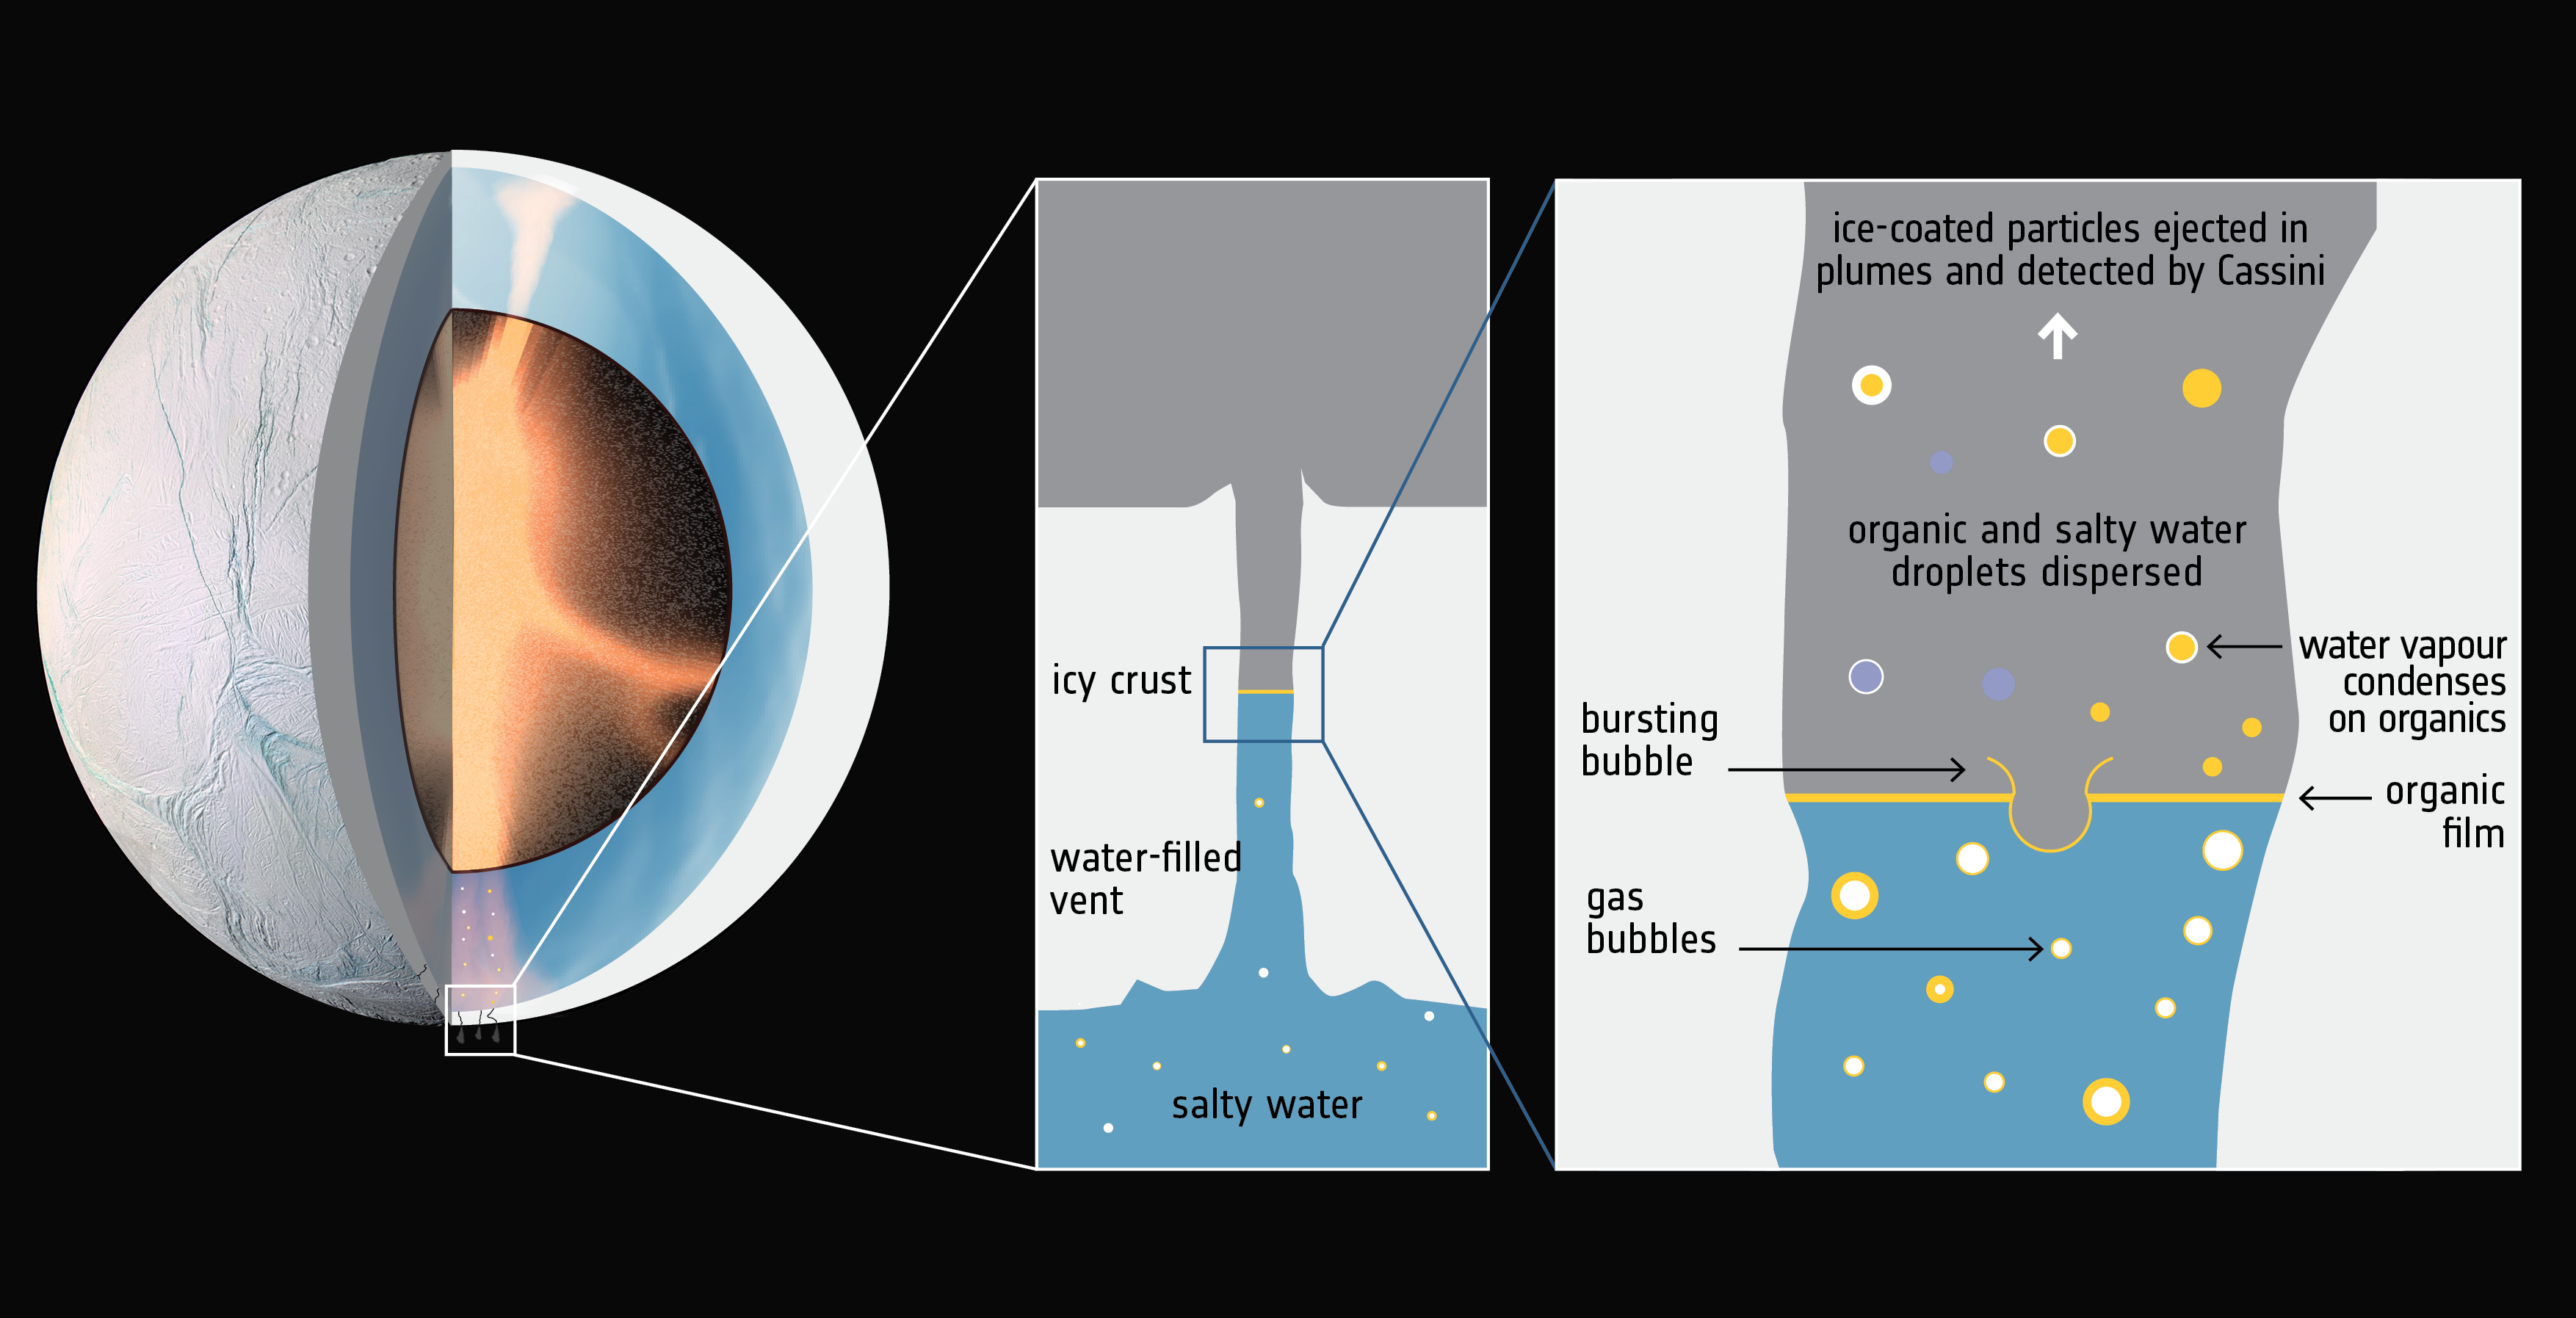
\includegraphics[width=0.9\textwidth]{enceladus-2.jpg}

\small {\it F. Postberg et al / the European Space Agency}

\EC
}
\frame{\frametitle{\bf Saturn from Cassini}
\BC
\normalsize Saturn has always been an emblem of the fascination of space... 

\BS

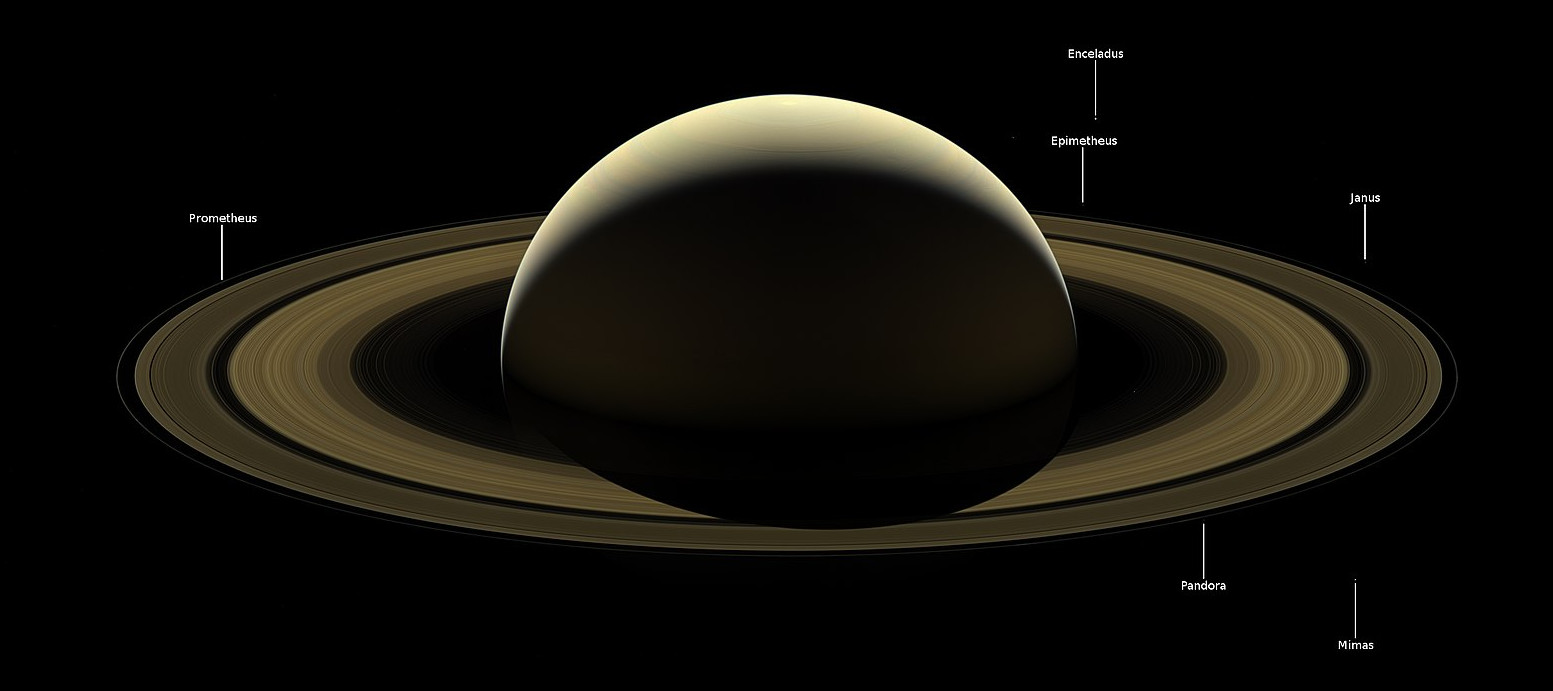
\includegraphics[width=\textwidth]{enceladus-4.jpg}

\BS\pause

... but now that we know more ...

\EC
}



\frame{\frametitle{\bf Exobiology: the search for water}
\BC
\large
Life on Earth needs liquid water; it allows molecules to float around and find each other
\EC

\BS
\BBC
\HC
Liquid water in the Solar System:

\BI
\item Need temperatures from 0-c. 100 C
\item Earth is perfect (we knew that)
\item Young Mars?
\item The moons of Jupiter and Saturn...
\item \color{Red} Most exciting near-term astrobiology experiment: send a probe to break through
the crust of one of these moons!
\EI

\HC
\BC
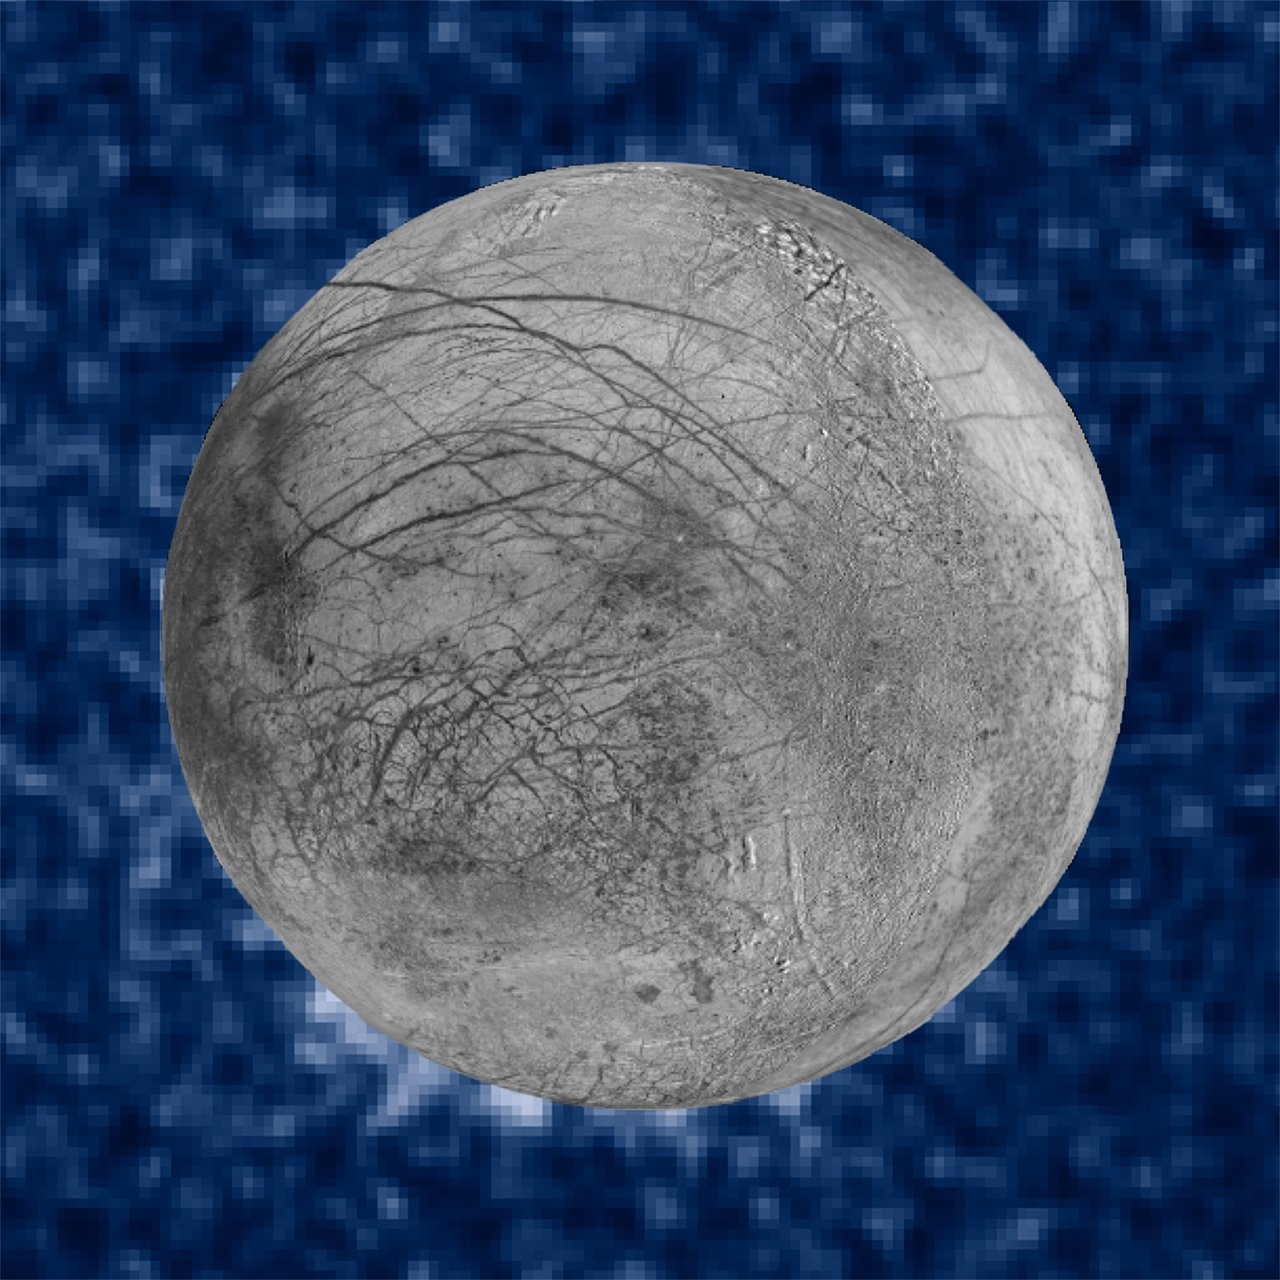
\includegraphics[width=.9\textwidth]{europa-plumes.jpg}\\
\it \footnotesize Galileo/Voyager/Hubble: ESA (2014)
\EC
\EEC
}

\frame{\frametitle{\bf Exobiology: encouraging signs from Earth}
\large
Life evolved on Earth very, very early in its history...
\BC
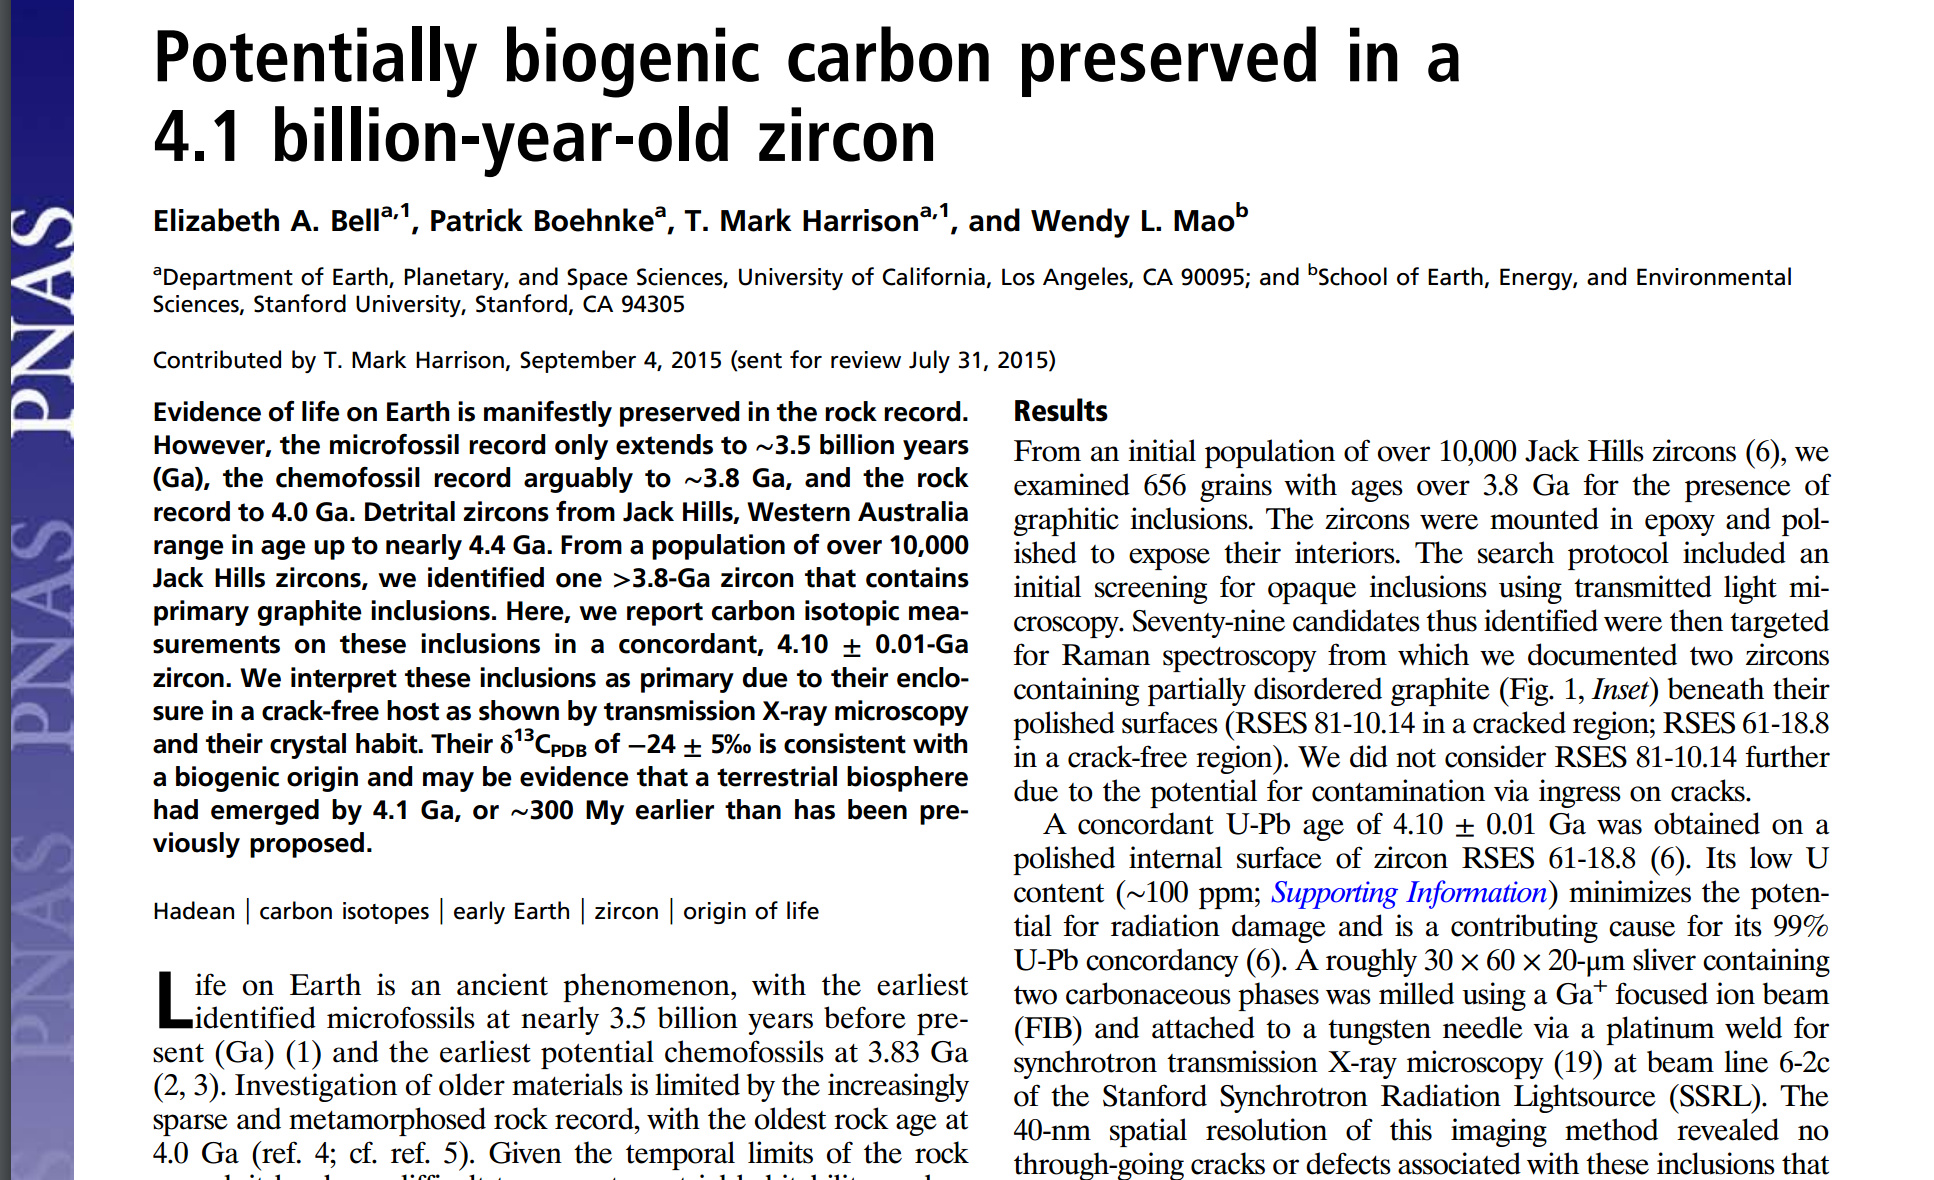
\includegraphics[width=0.8\textwidth]{pnas.jpg}
\EC
\begin{flushright}... this suggests that wherever life {\it can} develop, it will!\end{flushright}
}

\frame{\frametitle{\bf Extraterrestrial civilizations: different, but alike}
\large
Intelligent life elsewhere has the same resources we do -- the same chemical elements and the same physics.

\BS

Any intelligent beings in the Universe will come to many of same conclusions we have about Nature.

\BS

We'd probably see them in the same way we see everything else: light (radio signals).

}

%\frame{\frametitle{\bf Extraterrestrial civilizations: the Drake equation}
%
%How many extraterrestrial civilizations might there be? Frank Drake suggested that we multiply...
%
%\BI
%\item The number of stars per year that form \pause
%\item What fraction of those have planets (we think most of them, now) \pause
%\item What fraction of those planets could have liquid water and support life \pause
%\item What fraction of those planets probably {\it do} develop life \pause
%\item What fraction of ecologies evolve civilization \pause
%\item What fraction of civilizations emit strong radio signals (or something else) \pause
%\item The length of time that they do this (before ... what?) \pause
%\EI
%
%These quantities are all uncertain, and their product is {\it very} uncertain!
%
%\BS
%
%It's unlikely that we're the only life in the Universe. We might be the only broadcasting civilization in the Galaxy, though...
%
%\BS
%}

\frame{\frametitle{\bf Extraterrestrial civilizations: the Fermi paradox}

``It's likely they're out there, and that they're older than us. Then where are they?''

\BS

Lots of answers, all of them speculative, some of them depressing...

\BI
\item Civilizations tend not to last very long...
\item Civilizations are actually pretty rare
\item They're there, but aren't very advanced: humans are uniquely intelligent
\item They're there, but are {\it very} advanced and can hide from us
\item Nobody thinks we're worth talking to
\item ...
\EI
}


\frame{\frametitle{\bf Human travel to Mars and beyond}
\large
The problem with human travel: humans are fragile. Humans require life-support baggage and want to come home; robots don't.
\normalsize

\BS

Going to Mars is just within the reach of current technology (it's an economics problem, not a science one)
\BI
\item Mission of several years (there and back)
\item Providing for food, life support, and radiation shielding would be an engineering challenge, but we can do that
\item Would need rockets larger than Saturn V, but not impossibly so
\item Several clever ways to use robotics to reduce the size of the rockets needed (Mars Direct)
\EI

\BS

Going beyond would likely require substantial improvements in rockets.

\BS

Remember: a small improvement in exhaust velocity gives an exponential increase in how fast a rocket can make you go (and where you can go with it)
}

\frame{\frametitle{\bf Robots to the stars (that survive the trip)}
\large
{\it Voyagers} 1 and 2 are headed for the stars, but won't make it near any for tens of thousands of years.

\BS

$\rightarrow$ Can we send a probe to the stars, like {\it Viking} or {\it Spirit}?

\BS

The problem here is {\it time}. We could send a probe to Alpha Centauri now -- 4.3 ly (270,000 AU away). Should we?

\BS
\pause
Two options: 

\BI
\item A slow probe and patience: centuries or millennia 
\item Higher exhaust-velocity rockets
\pause
\item This would still take decades to a century
\item \bf The round-trip communication time would still be eight years!
\EI
}

\frame{\frametitle{\bf Improving rockets}
\large
Lots of ideas here -- some speculative, some tested (ask if you're curious!):
\BI 
\item \color{Red}Scramjets
%\BI 
%\item Harvest oxygen from Earth's atmosphere during initial escape-from-Earth rocket burn; it's much heavier than the hydrogen that goes with it
%\item Precursor idea already used for Eurofighter's air-to-air missiles ({\it Meteor})
%\EI
\item Nuclear rockets
%\BI
%\item A nuclear reactor can heat propellant to a higher temperature than its own chemical energy
%\item Probably the most tested of any of these (idea dates to the 1950's)
%\EI
\item Nuclear pulse propulsion
%\BI
%\item Set off nuclear explosives behind the armored rear of a spacecraft
%\item Only usable for huge spacecraft without laser fusion 
%\EI
\item Ion engines
%\BI
%\item Low thrust per weight, but consumes very little reaction mass (high exhaust velocity)
%\item Can't use to escape from Earth, but maybe on a space probe
%\EI
\item Solar sails
%\BI
%\item Sail on the solar wind, or on a laser from Earth or Earth orbit?
%\EI
\EI
}

\frame{\frametitle{\bf Improving humans and changing our outlook}
With only a little improvement in rockets, we can conquer space.

\BS

Science-fiction authors dream of ``faster-than-light travel'', but this is likely not possible. 

\BS

If we take to the stars, humans will be possibly be born, grow, live, love, and die in space. If we stay there long,
we will no doubt evolve to match our new surroundings...

\BS

There are ways to cheat: cryogenics, freezing embryos and trusting robots to teach babies how to be human...

\BS

Even then, a mission to Alpha Centauri is a mission that will outlive those that send it.

\BS

The greatest challenge in spacefaring won't be engineering, science, or even economics -- it will be {\it philosophy}.
}

\frame{\frametitle{\bf Improving humans and changing our outlook}
We are a young civilization.

\BS

Imagine that the distance from San Francisco to Syracuse was the history of Earth: 4500 km to 4.5 billion years.
\pause
\small
\BI
\item Life evolved somewhere around Reno, Nevada
\pause
\item Life created the oxygen atmosphere near Denver, Colorado (mass extinction!)
\pause
\item Sex was invented at Fermilab, Illinois (near Chicago) 
\pause
\item Life colonized the land at the westernmost edge of New York State
\pause
\item Dinosaurs lasted from Buffalo to Seneca Falls
\pause
\item We learned to walk on two legs at the Syracuse city limits (7 km)
\pause
\item We learned to cook at the War Memorial / Symphony Hall (2 km)
\pause
\item Modern humans evolved at the Hall of Languages (200 m)
\EI
}

\frame{\frametitle{\bf Improving humans and changing our outlook}
We are a young civilization.

\BS

Imagine that the distance from San Francisco to Syracuse was the history of Earth: 4500 km to 4.5 billion years.
\small
\BI
\item We left Africa at the entrance to Hendricks Chapel (50 m)
\pause
\item We invented agriculture on the other side of this room (10 m)
\pause
\item Ptolemy wrote the {\it Almagest} a handspan away (2 m)
\pause
\item da Vinci dreamed of flight 60 cm away
\pause
\item Newton wrote the {\it Principia} 40 cm away
\pause
\item Tsiolkovsky explained rocketry only a handspan away
\pause
\item We landed on the Moon a thumb-length away
\pause
\item You were born an inch away, and I was an inch and a half
\pause
\item Barack Obama was president half of the width of a pencil ago
\pause
\item You started this class only the thickness of a fingernail ago
\EI
}

\frame{\frametitle{\bf Improving humans and changing our outlook}

\large

We can conquer space; to become a spacefaring civilization, we will likely need to conquer time as well.

\pause

\normalsize

\BS
\BS
\it
``I want to build a clock that ticks once a year. The century hand advances once every one hundred years, and the cuckoo comes out on the millennium. I want the cuckoo to come out every millennium for the next 10,000 years. If I hurry I should finish the clock in time to see the cuckoo come out for the first time.'' 

\BS
\begin{flushright}\rm --Danny Hillis, of the Long Now Foundation, 01995\end{flushright}
}


\frame{

\large

\it

``The oldest and strongest emotion of mankind is fear, and the oldest and strongest kind of fear is fear of the unknown.''

\begin{flushright}
	\rm -H. P. Lovecraft, 1927
\end{flushright}

\BS\BS\BS


``We live on a placid island of ignorance in the midst of black seas of infinity, and it was not meant that we should voyage far. The sciences, each straining in its own direction, have hitherto harmed us little; but some day the piecing together of dissociated knowledge will open up such terrifying vistas of reality, and of our frightful position therein, that we shall either go mad from the revelation or flee from the deadly light into the peace and safety of a new dark age.''


\begin{flushright}
	\rm -H. P. Lovecraft, 1926, from {\it The Call of Cthulhu}
\end{flushright}

}


\frame{\frametitle{\bf \large We end where we begun: humility and empowerment}
\BCC
\column{0.45\textwidth}
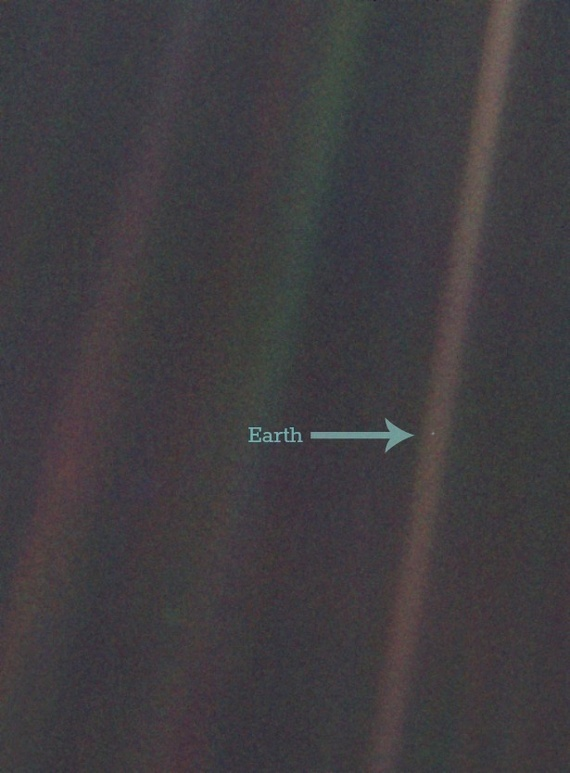
\includegraphics[width=\textwidth]{pale-blue-dot.jpg}
\column{0.55\textwidth}

\scriptsize

``Consider again that dot. That's here. That's home. That's us. On it everyone you love, everyone you know, everyone you ever heard of, every human being who ever was, lived out their lives. The aggregate of our joy and suffering, thousands of confident religions, ideologies, and economic doctrines, every hunter and forager, every hero and coward, every creator and destroyer of civilization, every king and peasant, every young couple in love, every mother and father, hopeful child, inventor and explorer, every teacher of morals, every corrupt politician, every "superstar", every "supreme leader", every saint and sinner in the history of our species lived there -- on a mote of dust suspended in a sunbeam.

\medskip\BS

The Earth is a very small stage in a vast cosmic arena. Think of the rivers of blood spilled by all those generals and emperors so that, in glory and triumph, they could become the momentary masters of a fraction of a dot. Think of the endless cruelties visited by the inhabitants of one corner of this pixel on the scarcely distinguishable inhabitants of some other corner, how frequent their misunderstandings, how eager they are to kill one another, how fervent their hatreds.


\ECC
}


\frame{\frametitle{\bf \large We end where we begun: humility and empowerment}
\BCC
\column{0.45\textwidth}
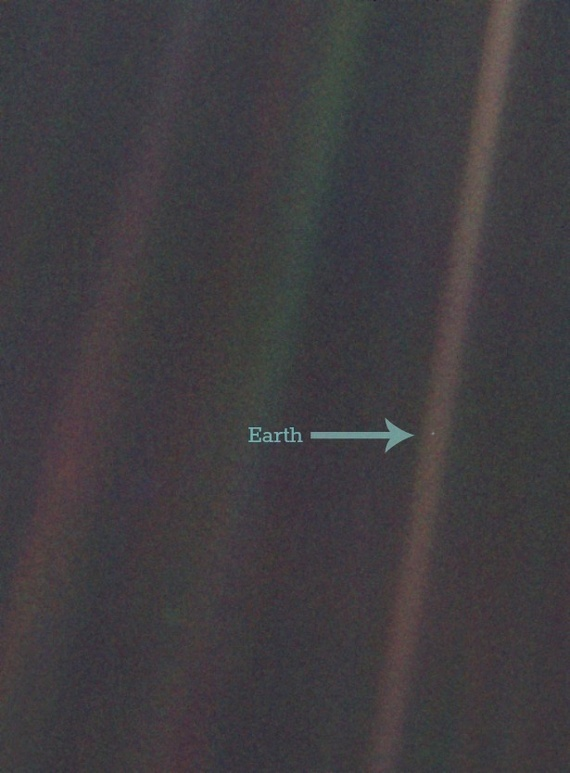
\includegraphics[width=\textwidth]{pale-blue-dot.jpg}
\column{0.55\textwidth}

\scriptsize


Our posturings, our imagined self-importance, the delusion that we have some privileged position in the Universe, are challenged by this point of pale light. Our planet is a lonely speck in the great enveloping cosmic dark....

\medskip

The Earth is the only world known so far to harbor life. There is nowhere else, at least in the near future, to which our species could migrate. Visit, yes. Settle, not yet. Like it or not, for the moment the Earth is where we make our stand.

\medskip

It has been said that astronomy is a humbling and character-building experience. There is perhaps no better demonstration of the folly of human conceits than this distant image of our tiny world. To me, it underscores our responsibility to deal more kindly with one another, and to preserve and cherish the pale blue dot, the only home we've ever known.''

\BS

\normalsize
\begin{flushright}--Carl Sagan, \it Pale Blue Dot (1994)\end{flushright}


\ECC
}

\frame{\frametitle{\bf \large We end where we begun: humility and empowerment}

But...

\BS

We can look at all of this, here from our little mote of dust...

\BS

... we can understand how it works -- we, our little carbon-and-water brains, can comprehend the steps in the dance that the Universe is dancing.

\BS

\pause

... and it's the same everywhere. We -- our star, our planet, and our bodies -- are part of it, and we can fathom how it works.

\pause
\BS
So, if our bodies and our planet are very small -- how much our minds can accomplish!
}

\frame{\frametitle{\bf Course evaluations}
\BC


You have gotten an email regarding course evaluations for the University.

\BS
\BS

We take this feedback seriously; I, as a new professor, trying new things, am especially interested in what you have to say.

\BS

Thank you for your patience as I've tried different things, seen what you all like, and what you don't.

\BS

Please tell me and my supervisors what you think of this course!
\EC

}


\frame{\frametitle{\bf Three last things (1/3): the challenge from Day 1}

\large
``With more knowledge comes deeper, more wonderful mystery...
with pleasure and confidence we turn over each new stone to find
unimagined strangeness leading on to more wonderful questions and mysteries--certainly
a grand adventure!

\bigskip

Our poets
do not write about [this]; our artists do not try to portray [it]. I don't know why.
{\bf Is nobody inspired by our present picture of the universe?} [Science] remains unsung
by singers, so you are reduced to hearing not a song or poem, but an evening lecture about it.
Is no one inspired by our present picture of the universe? {\bf This is not yet a
scientific age.}''

\bigskip
\bigskip

\begin{flushright}--Richard Feynman, from {\it The Value of Science} (1955)
\end{flushright}
}

\frame{\frametitle{\bf A scientific age? You bet.}
\BCC
\HC
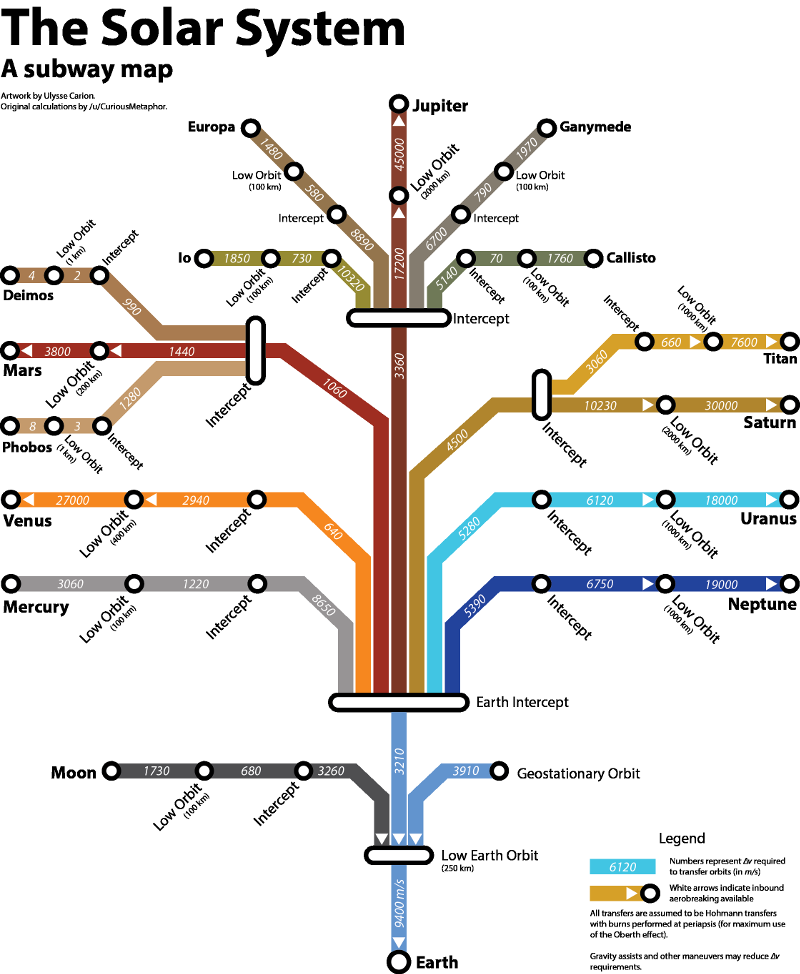
\includegraphics[width=\textwidth]{delta-v.png}
\HC
\large
\BC
This was made by a user on the ``space'' subreddit. (I verified some of the numbers.)
\EC
\ECC
}

\frame{\frametitle{\bf A scientific age? You bet.}
\BC
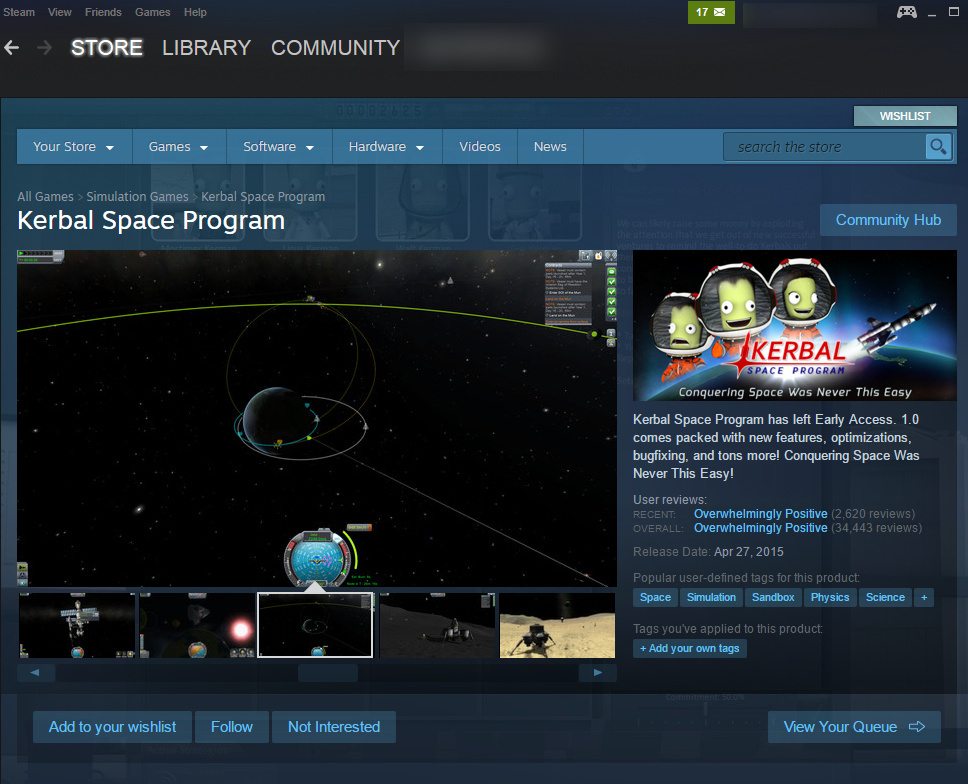
\includegraphics[width=0.6\textwidth]{kerbal.jpg}
\EC
\large

\BS

\BC
... and you can buy a very physically accurate simulation of spaceflight and rocketry on Steam!
\EC
}

\frame{\frametitle{\bf Going beyond (2/3)}

\Large

This has been a pretty broad survey of astronomy -- and much of physics!

\BS

What comes next, if you want more of this sort of thing? 
}

\frame{\frametitle{\bf Going beyond (2/3): Astronomy 104}



\large

Our class covered astronomy inside the Solar System.

\BS

AST104 covers the rest of the Universe:

\BI
\item The life and death of stars
\item Galaxies
\item Neutron stars
\item Black holes
\item Gravitational waves
\item The origin and fate of the Universe
\EI

... the really awesome stuff!

\BS

It'll be taught next semester by {\color{Red}Prof. Denver Whittington},
who is an entertaining teacher and a great fellow. (Ask him about the time 
we melted things trying to work on the telescope in Holden!)

}

\frame{\frametitle{\bf Going beyond (2/3): ... and more}
\BS

\Large
\BC We have an (astro)physics major/minor! \EC


\BS
\large

Courses in...

\BI
\normalsize
\item Astrophysics and the lives of stars
\item Relativity and cosmology
\item Waves, vibrations, and optics
\item Quantum mechanics
\item Computer modeling and simulation
\item The physics of heat 
\item Teaching physics
\item The physics of living things
\EI
\pause

A degree in physics is a highly-valued thing in industry -- you can study the stars and the natural world, and then have a great shot at a good job.

\BS
\BC
\color{Red}If you're interested in pursuing this, come speak to me!
\EC
}

\frame{\frametitle{\bf Inspiration (3/3)}

\large

When I was asked to teach this class, Patty Whitmore (then academic coordinator) told me: ``These folks aren't here to learn mathematics. They're not here to learn 
only the laws of physics; they're here to learn what science is about.''

\BS\BS

In this class I've aimed to both teach you a little astronomy, and how to think scientifically ... but, also, to connect astronomy to the broader
story of human thought.

\BS\BS\pause

In the end, we look at the sky because it's beautiful -- and because it's inspiring.

}

\frame{


Last year, I ended this class with a poem by James Agee about the beauty of the 
night sky, which was set to music by Morton Lauridsen. 

\BS\BS\pause

I played a faraway man's music and showed a dead man's poem.

\BS\BS\pause

We took the final exam.

\BS\BS\pause

And then Ohana and I worked for {\it days} looking at and grading your final projects. So many of them were {\it stunning}.

\BS\BS\pause

But, on the 27th of December, exhausted and both sick from eating nothing but pizza for two days, we arrived at Annie Shi's -- and it is with her words that I'd like to end this year's class.

\BS\BS\pause

\url{https://edelwysse.wixsite.com/ast101}

\BS\BS\pause

Thank you, Annie. \tt <3

}
%
%\frame{
%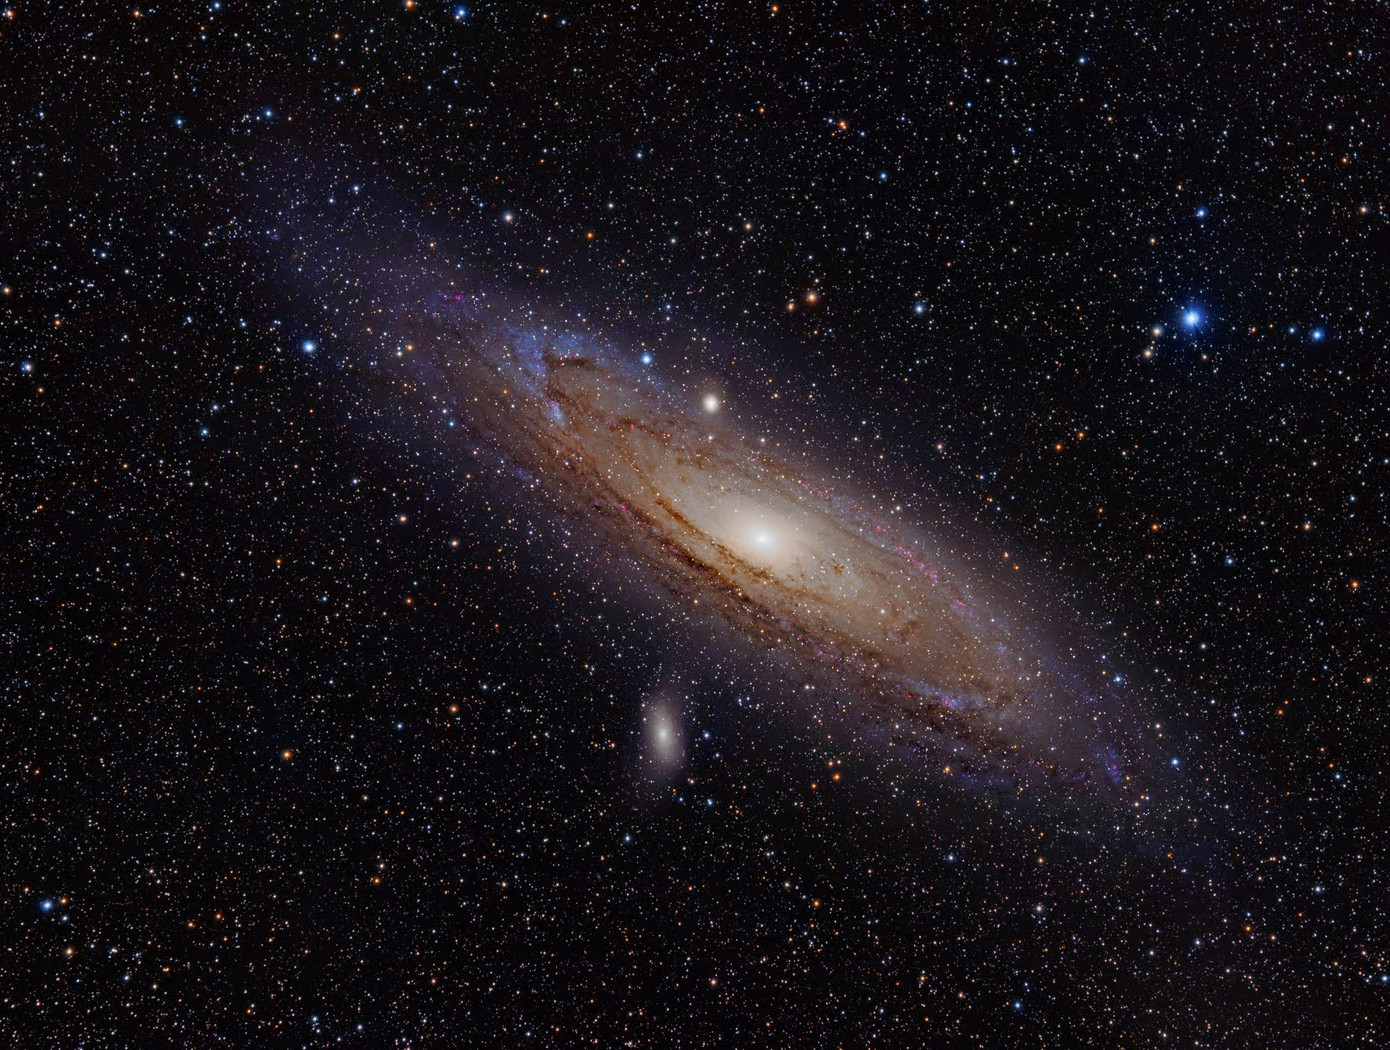
\includegraphics[height=\paperheight]{andromeda.jpg}
%}
%
%\frame{
%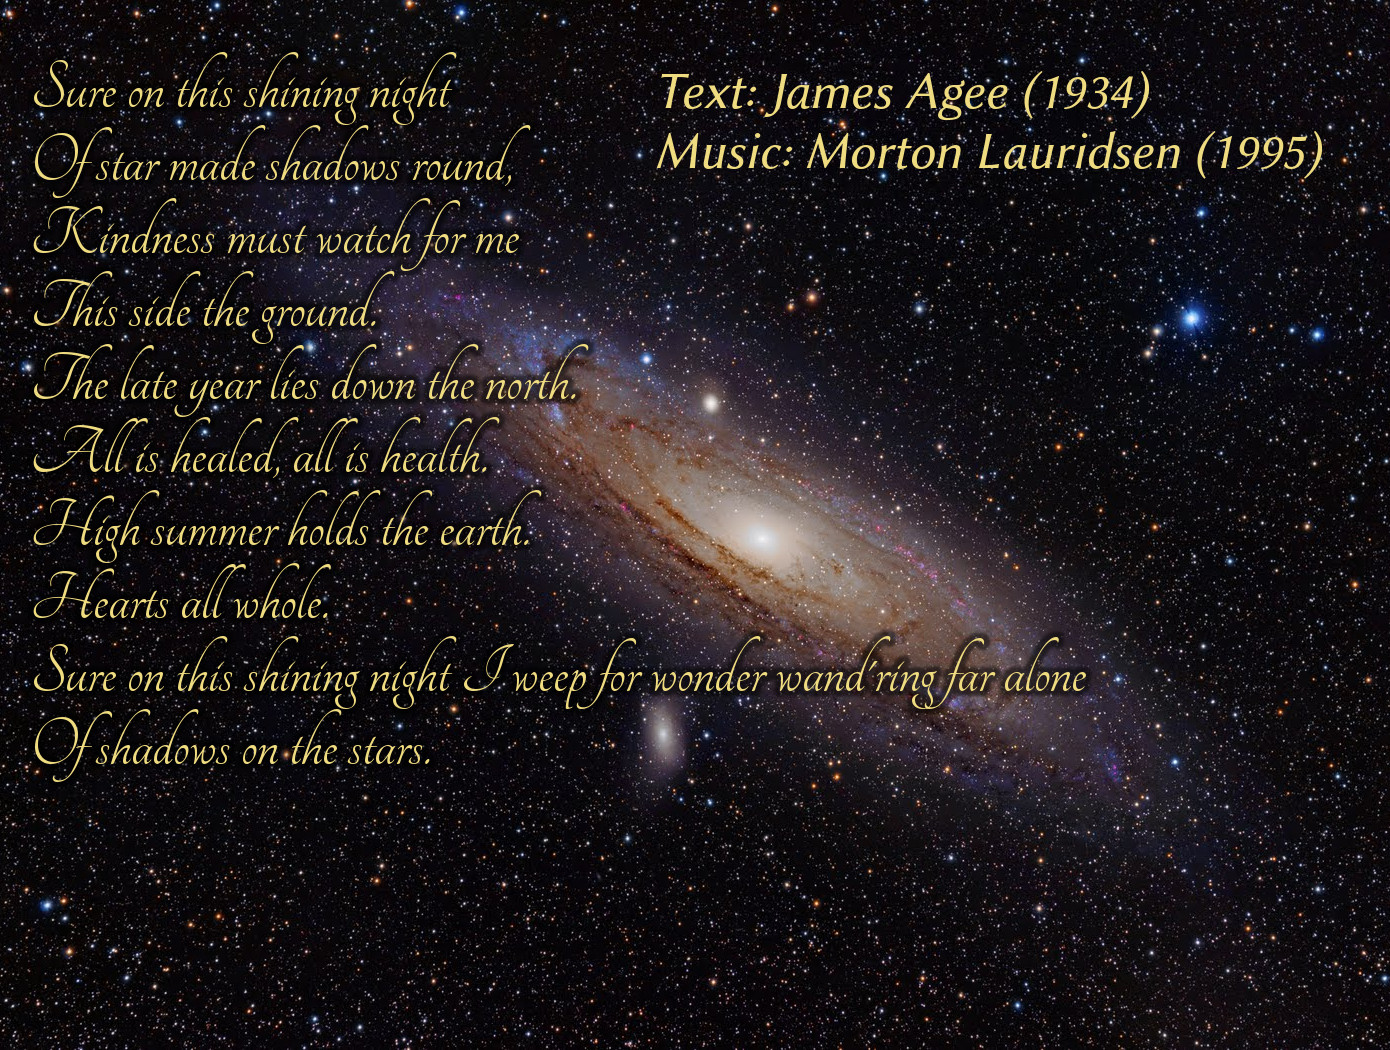
\includegraphics[height=\paperheight]{andromeda-annotated-first.jpg}
%}
%
%\frame{
%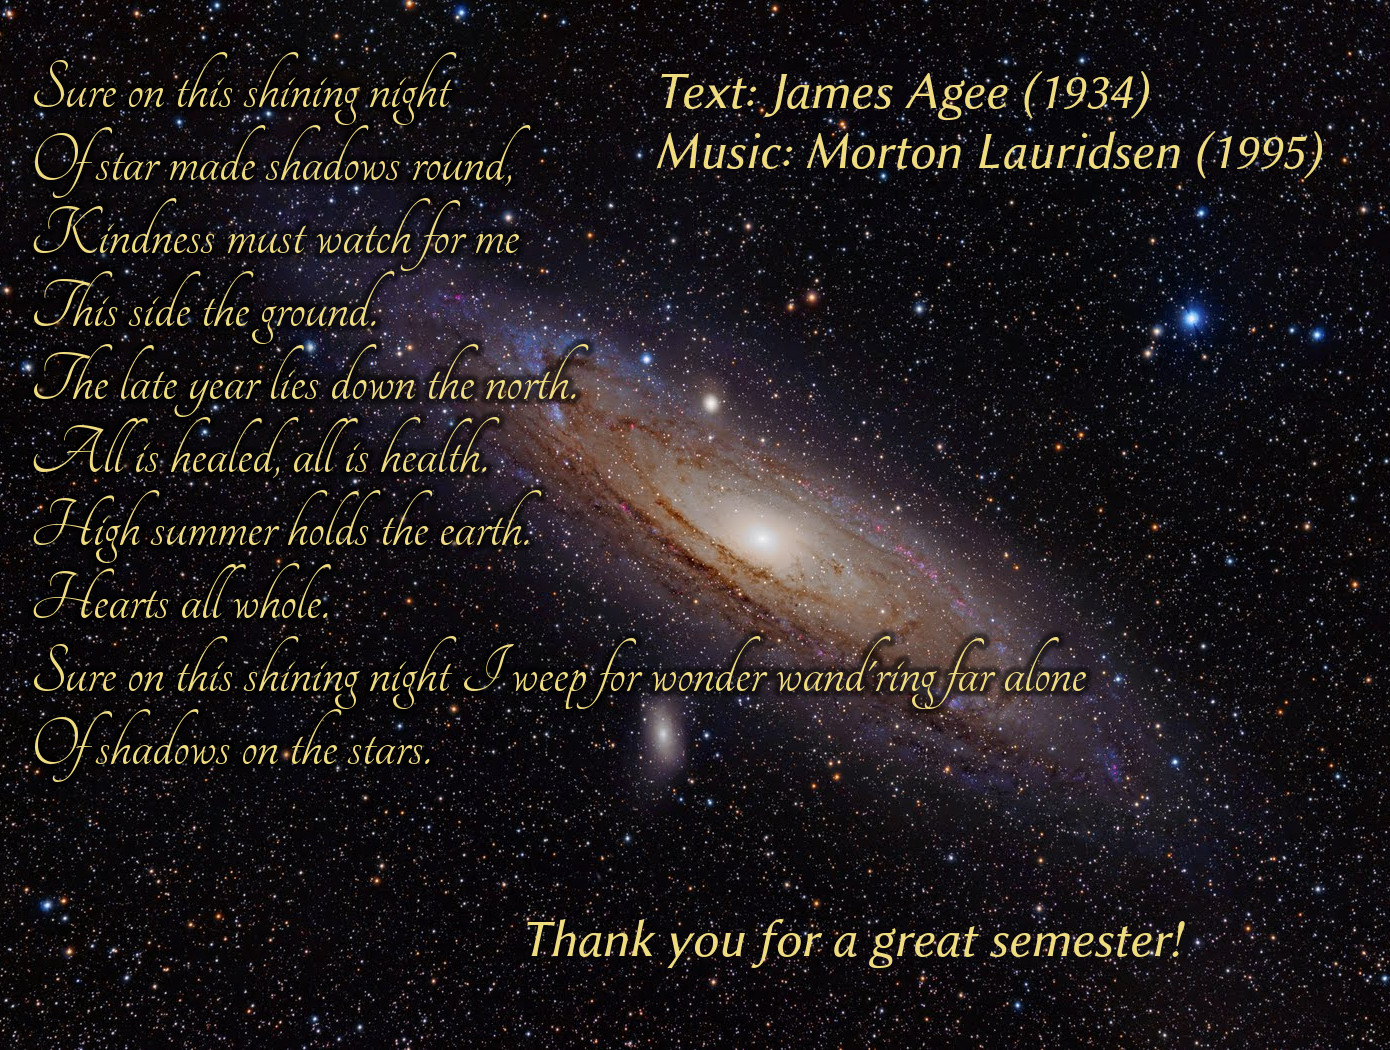
\includegraphics[height=\paperheight]{andromeda-annotated.jpg}
%}
%{ % all template changes are local to this group.
%    \setbeamertemplate{navigation symbols}{}
%    \begin{frame}[plain]
%        \begin{tikzpicture}[remember picture,overlay]
%            \node[at=(current page.center)] {
%                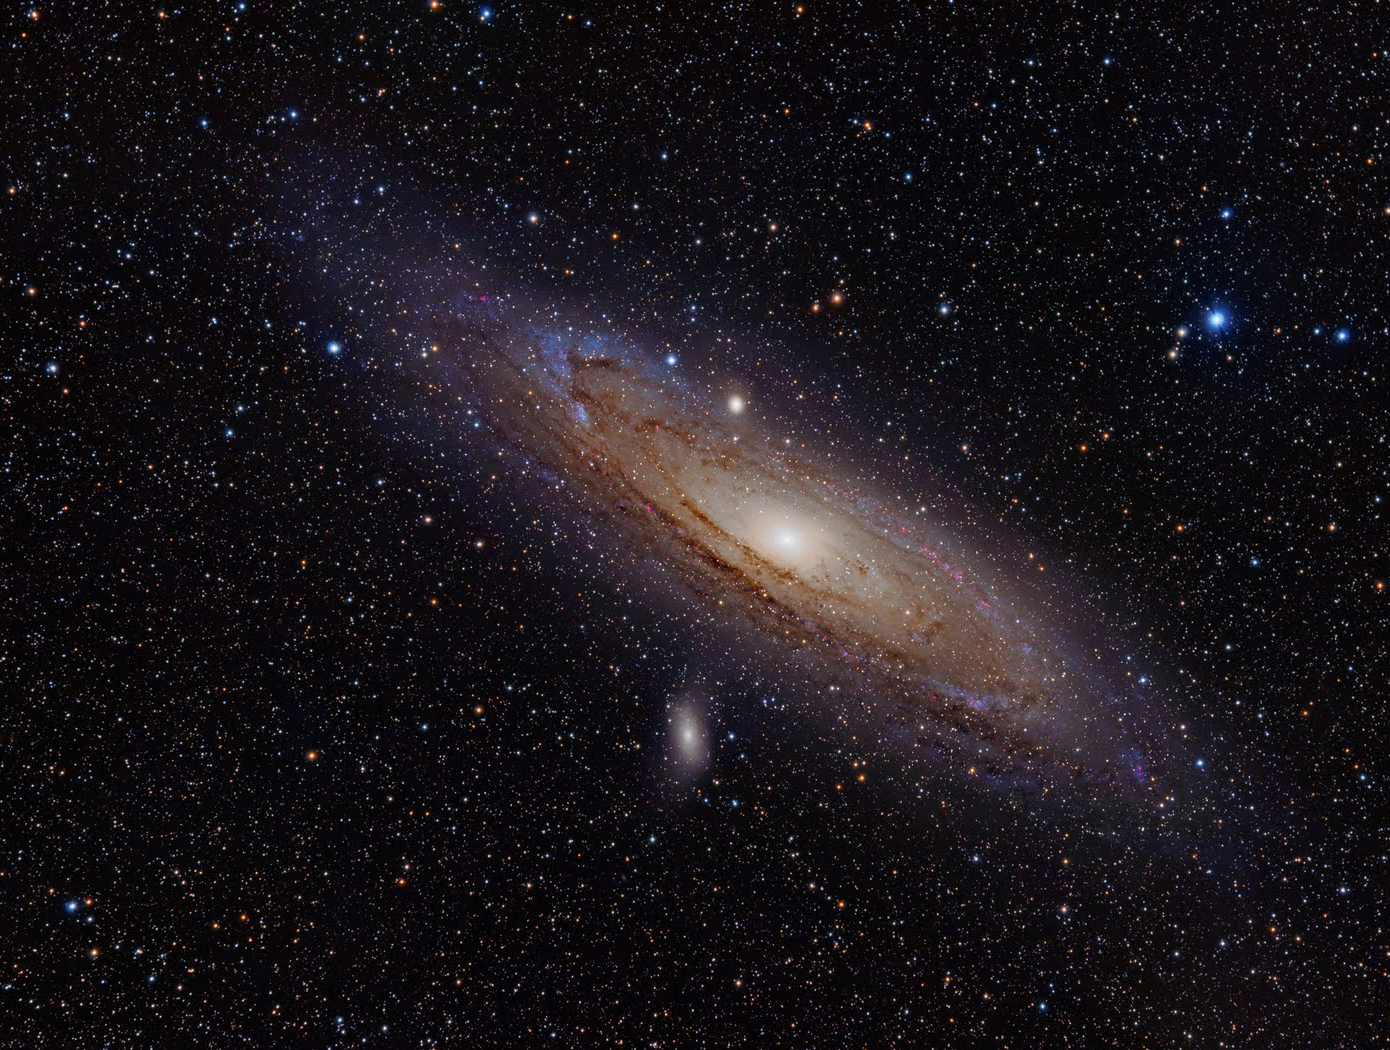
\includegraphics[height=\paperheight]{andromeda-1.png}
%            };
%        \end{tikzpicture}
%     \end{frame}
%}
%
%{ % all template changes are local to this group.
%    \setbeamertemplate{navigation symbols}{}
%    \begin{frame}[plain]
%        \begin{tikzpicture}[remember picture,overlay]
%            \node[at=(current page.center)] {
%                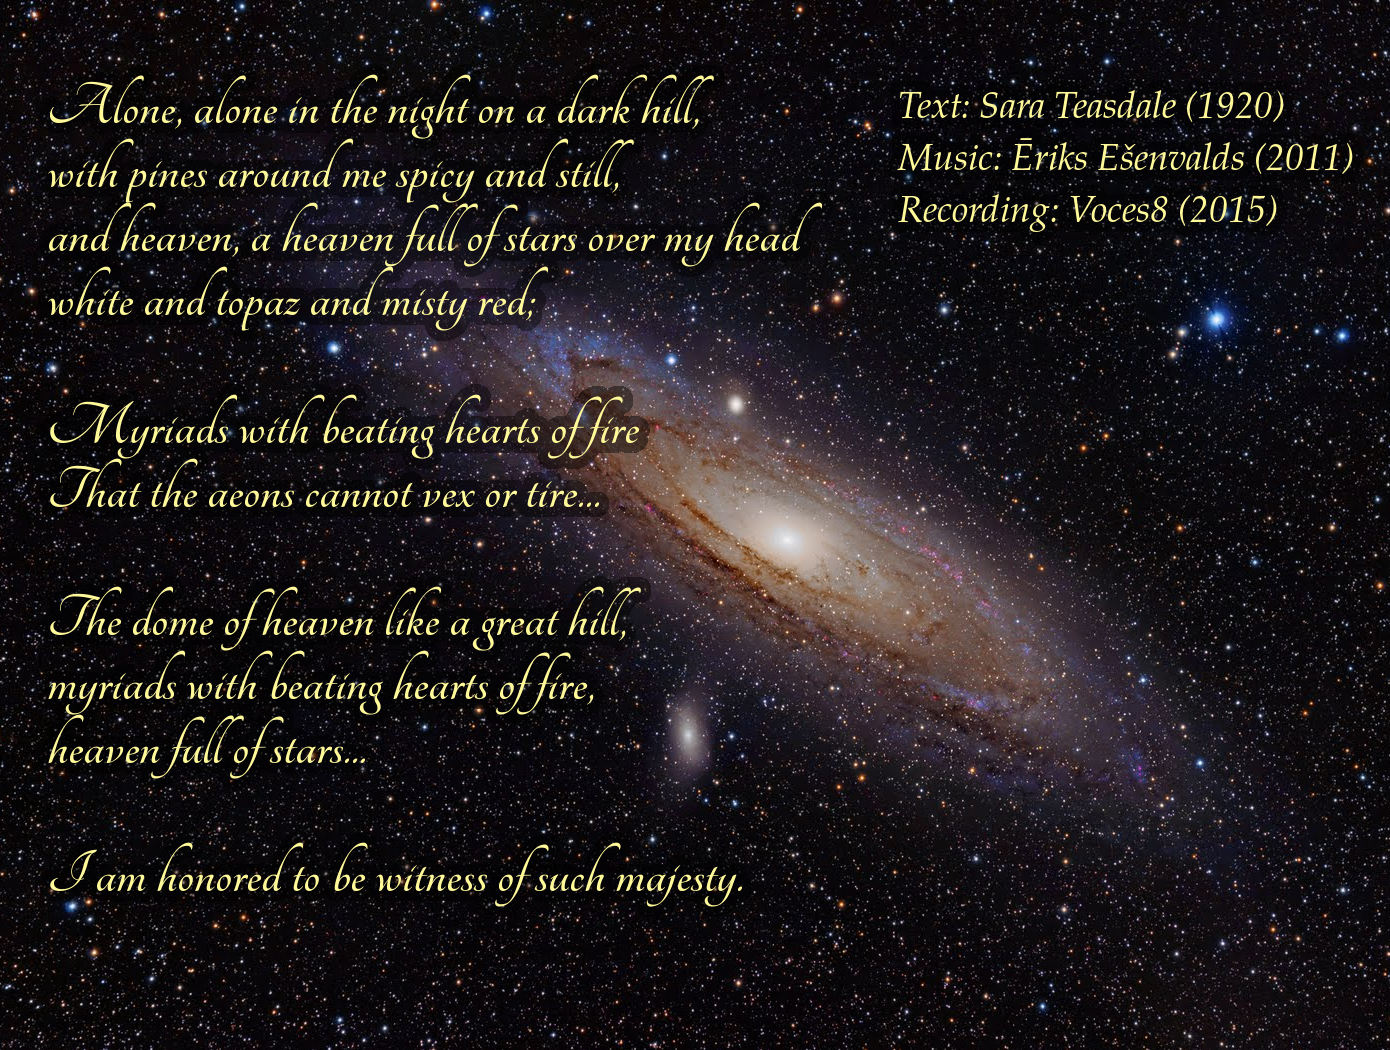
\includegraphics[height=\paperheight]{andromeda-2.png}
%            };
%        \end{tikzpicture}
%     \end{frame}
%}
%
{ % all template changes are local to this group.
    \setbeamertemplate{navigation symbols}{}
    \begin{frame}[plain]
        \begin{tikzpicture}[remember picture,overlay]
            \node[at=(current page.center)] {
                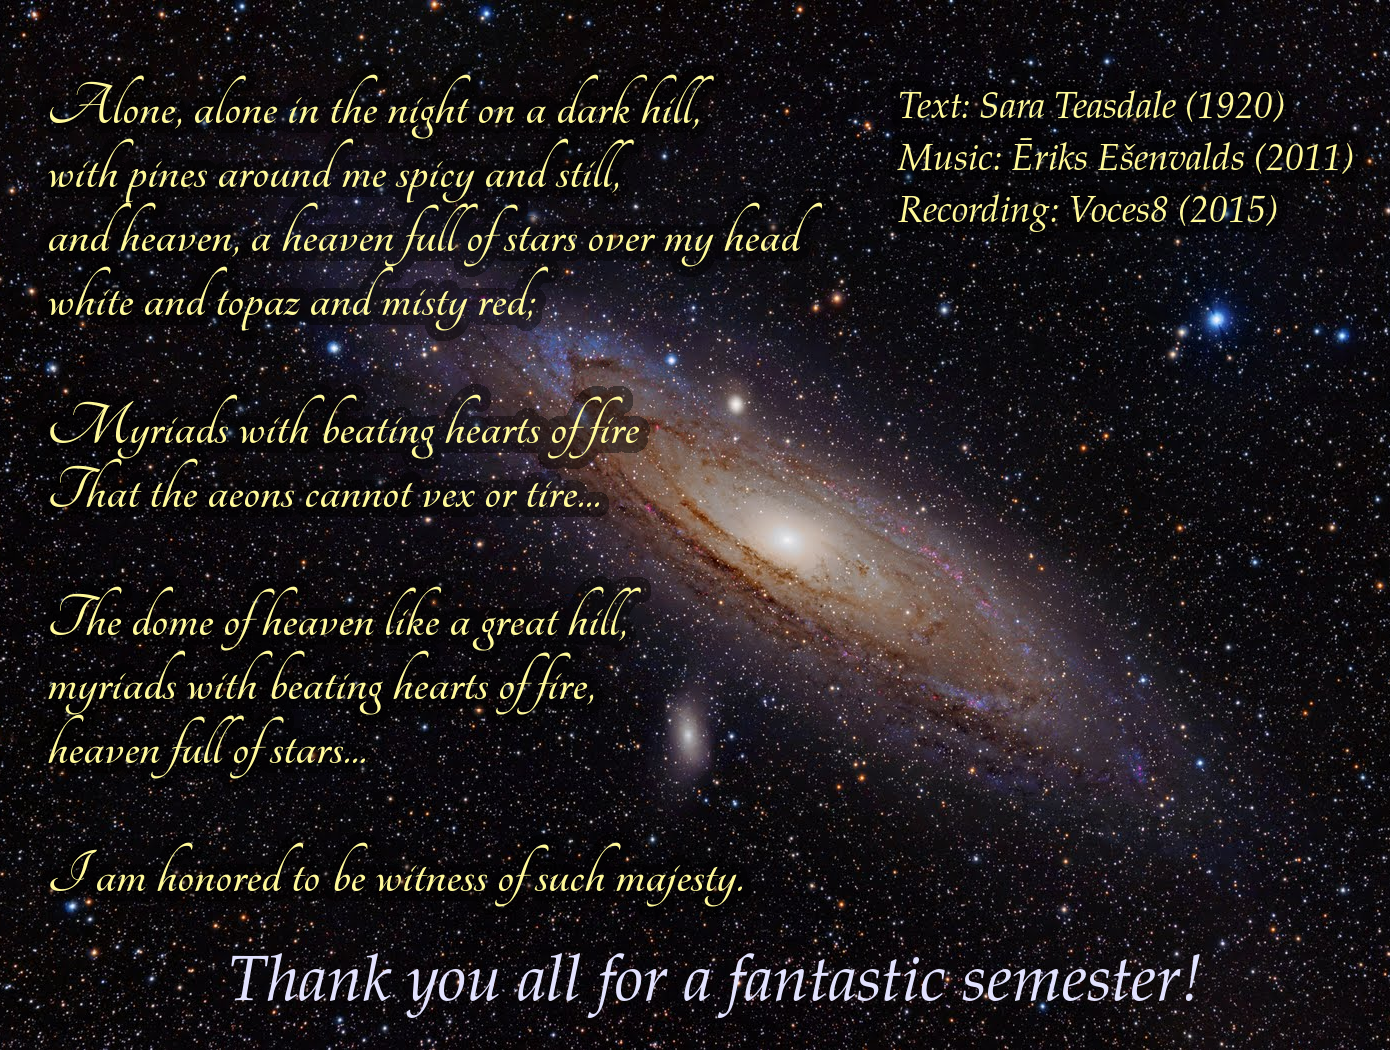
\includegraphics[height=\paperheight]{andromeda-3.png}
            };
        \end{tikzpicture}
     \end{frame}
}







\end{document}
